%%%%%%%%%%%%%%%%%%%%%%%%%%%%%%%%%%%%%%%%%%%%%%%%%%%%%%%%%%%%%%%%%%%%
%% I, the copyright holder of this work, release this work into the
%% public domain. This applies worldwide. In some countries this may
%% not be legally possible; if so: I grant anyone the right to use
%% this work for any purpose, without any conditions, unless such
%% conditions are required by law.
%%%%%%%%%%%%%%%%%%%%%%%%%%%%%%%%%%%%%%%%%%%%%%%%%%%%%%%%%%%%%%%%%%%%

\documentclass[
  digital, %% The `digital` option enables the default options for the
           %% digital version of a document. Replace with `printed`
           %% to enable the default options for the printed version
           %% of a document.
  color,   %% Uncomment these lines (by removing the %% at the
           %% beginning) to use color in the printed version of your
           %% document
  oneside, %% The `oneside` option enables one-sided typesetting,
           %% which is preferred if you are only going to submit a
           %% digital version of your thesis. Replace with `twoside`
           %% for double-sided typesetting if you are planning to
           %% also print your thesis. For double-sided typesetting,
           %% use at least 120 g/m² paper to prevent show-through.
  lof,     %% The `lof` option prints the List of Figures. Replace
           %% with `nolof` to hide the List of Figures.
  nolot,     %% The `lot` option prints the List of Tables. Replace
           %% with `nolot` to hide the List of Tables.
]{fithesis4}
%% The following section sets up the locales used in the thesis.
\usepackage[resetfonts]{cmap} %% We need to load the T2A font encoding
\usepackage[T1,T2A]{fontenc}  %% to use the Cyrillic fonts with Russian texts.
\usepackage[
  main=english, %% By using `czech` or `slovak` as the main locale
                %% instead of `english`, you can typeset the thesis
                %% in either Czech or Slovak, respectively.
  english %% The additional keys allow
]{babel}        %% foreign texts to be typeset as follows:
%%
%%   \begin{otherlanguage}{german}  ... \end{otherlanguage}
%%   \begin{otherlanguage}{russian} ... \end{otherlanguage}
%%   \begin{otherlanguage}{czech}   ... \end{otherlanguage}
%%   \begin{otherlanguage}{slovak}  ... \end{otherlanguage}
%%
%% For non-Latin scripts, it may be necessary to load additional
%% fonts:
% \usepackage{paratype}
% \def\textrussian#1{{\usefont{T2A}{PTSerif-TLF}{m}{rm}#1}}
%%
%% The following section sets up the metadata of the thesis.
\thesissetup{
    date        = \the\year/\the\month/\the\day,
    university  = mu,
    faculty     = fi,
    type        = bc,
    department  = Department of Computer Systems and Communications,
    author      = Jakub Maloštík,
    gender      = m,
    advisor     = {Ing. Milan Brož, Ph.D.},
    title       = {Disk sector content analysis and visualization},
    TeXtitle    = {Disk sector content analysis and visualization},
    keywords    = {visualization, disk encryption, disk sector, randomness detection},
    TeXkeywords = {visualization, disk encryption, disk sector, randomness detection},
    abstract    = {%
      Data visualization is often vital for people's understanding of the data.
      This thesis discusses methods of classifying the sectors based on their randomness using statistical tests or Shannon's entropy calculation and methods for visualization and introduces a utility that analyzes sectors of a provided disk image and visualizes them to provide a visual representation of which sectors are encrypted, discarded, or may contain readable data.
      Then, several examples of disk images visualized using the introduced utility are showcased and discussed.
    },
    thanks      = {%
      These are the acknowledgements for my thesis, which can

      span multiple paragraphs.
    },
    bib         = bibliography.bib,
    %% Remove the following line to use the JVS 2018 faculty logo.
    facultyLogo = fithesis-fi,
}
\usepackage{makeidx}      %% The `makeidx` package contains
\makeindex                %% helper commands for index typesetting.
\usepackage[acronym]{glossaries}          %% The `glossaries` package
\renewcommand*\glspostdescription{\hfill} %% contains helper commands
\loadglsentries{example-terms-abbrs.tex}  %% for typesetting glossaries
%\makenoidxglossaries                      %% and lists of abbreviations.
%% These additional packages are used within the document:
\usepackage{paralist} %% Compact list environments
\usepackage{amsmath}  %% Mathematics
\usepackage{amsthm}
\usepackage{amsfonts}
\usepackage{url}      %% Hyperlinks
\usepackage{markdown} %% Lightweight markup
\usepackage{listings} %% Source code highlighting
\lstset{
  basicstyle      = \ttfamily,
  identifierstyle = \color{black},
  keywordstyle    = \color{blue},
  keywordstyle    = {[2]\color{cyan}},
  keywordstyle    = {[3]\color{olive}},
  stringstyle     = \color{teal},
  commentstyle    = \itshape\color{magenta},
  breaklines      = true,
}
\usepackage{caption}
\usepackage[font=normalsize]{subcaption}
\usepackage{floatrow} %% Putting captions above tables
\floatsetup[table]{capposition=top}
\usepackage[babel]{csquotes} %% Context-sensitive quotation marks

\graphicspath{{figures}} %% change to figures-orig-res for figures that weren't downsized

\hyphenation{Vera-Crypt}

\begin{document}
%% Uncomment the following lines (by removing the %% at the beginning)
%% and to print out List of Abbreviations and/or Glossary in your
%% document. Titles for these tables can be changed by replacing the
%% titles `Abbreviations` and `Glossary`, respectively.
%% \clearpage
%% \printnoidxglossary[title={Abbreviations}, type=\acronymtype]
%% \printnoidxglossary[title={Glossary}]

%% The \chapter* command can be used to produce unnumbered chapters:
\chapter*{Introduction}
\label{chap:introduction}
%% Unlike \chapter, \chapter* does not update the headings and does not
%% enter the chapter to the table of contents. I we want correct
%% headings and a table of contents entry, we must add them manually:
\markright{\textsc{Introduction}}
\addcontentsline{toc}{chapter}{Introduction}

Disks (e.g., hard drives, SSDs, Flash drives) are divided into atomic parts named sectors, which are represented as blocks in the software layer.
Sectors store a fixed amount of data, usually 512 bytes or 4KiB, but other sector sizes can be used.
Sectors may contain partition tables, file system information, files or be empty.

Sectors can contain specific byte patterns (e.g., be full of zeroes), which can be analyzed and used to identify the nature of the stored content.
When a byte pattern is not present, sector content can be analyzed for entropy to estimate whether it is encrypted.
A good way to get an idea about which parts of the disk are encrypted and where filesystem data is stored is to visualize this data.
This visualization will allow humans to distinguish between different data encryption methods such as file-hosted volumes and full disk encryption and even uncover flawed encryption.
Visualizing can also be very useful as an illustration while teaching.
 
The utility introduced in this bachelor's thesis analyzes the sectors of a user-specified size of a provided disk image and visualizes the result using the Pillow Python library.
The utility is also easily extensible by other output methods.

The text of this thesis is structured into five chapters.
Chapter number one explains the foundations of the thesis and examines prior work.
Chapter number two describes the used tools and technologies in the implementation.
Chapter number three describes the individual parts of the implementation and the options the implementation provides.
Chapter number four shows examples of images generated by the utility on various inputs.
The fifth and final chapter concludes with the evaluation of the implemented utility.

The resulting utility is available on GitHub\footnote{\url{https://github.com/malon43/entropy-visualization}} under the MIT License.
% Theses are rumoured to be \enquote{the capstones of education}, so
% I decided to write one of my own. If all goes well, I will soon
% have a diploma under my belt. Wish me luck!

% \begin{otherlanguage}{czech}
% Říká se, že závěrečné práce jsou \enquote{vyvrcholením studia}
% a tak jsem se rozhodl jednu také napsat. Pokud vše půjde podle
% plánu, odnesu si na konci semestru diplom. Držte mi palce!
% \end{otherlanguage}

% \begin{otherlanguage}{slovak}
% Hovorí sa, že záverečné práce sú \enquote{vyvrcholením štúdia}
% a tak som sa rozhodol jednu tiež napísať. Ak všetko pôjde podľa
% plánu, odnesiem si na konci semestra diplom. Držte mi palce!
% \end{otherlanguage}

% \begin{otherlanguage}{german}
% Man munkelt, dass die Dissertation \enquote{die Krönung der
% Ausbildung} ist. Deshalb habe ich mich beschlossen meine eigene
% zu schreiben. Wenn alles gut geht, bekomme ich bald ein Diplom.
% Wünsch mir Glück!
% \end{otherlanguage}

% \begin{otherlanguage}{russian}\textrussian{%
% Говорят, что тезис -- это \enquote{кульминация обучения}. Поэтому
% я и решил написать собственный тезис. Если всё сработает по плану,
% я скоро получу диплом. Желайте мне удачи!
% }\end{otherlanguage}

\chapter{Sector content visualization}
\label{chap:sector-content-visualization}

This review focuses on works on the topics of block pattern and encryption detection and ways of visualization

\section{Analysis}
\label{sec:analysis}

Each disk is divided into tens, even hundreds of millions of sectors.
Each disk sector stores some data.
Sectors of empty new drives would be mostly initialized with a pattern of zeroes, except for partitioning tables and file system metadata.

Most recent drives use 4KiB sized sectors, also known as Advanced Format, but still provide backward compatibility with older systems which expect 512B sector size with 512B sector size emulation. \cite{seagate} 

This section describes parts of analyzing the disk sectors.

\subsection{Block patterns}
\label{ssec:block-analysis}

Sector byte pattern is a specific configuration of bytes, which would indicate what this sector is used for.
For example, a repeated pattern of byte \texttt{x00} often signalizes that this sector has not been used yet, or that the blocks have been freed by the TRIM command.
The TRIM command is used by the software to inform the drive which sectors no longer contain user data in order to increase performance.\cite{mcmillen21}
Or, bytes \texttt{x55xAA} at the end of the sector would signalize a block containing master boot record (MBR).
However, while in many cases, analysis for positions of bytes is not as time-intensive as analysis of randomness or single-byte patterns, multiple problems show up:
\begin{itemize}
    \item Time spent testing for many positions, and byte configurations will add up.
    (The utility blkid \cite{blkid} and its underlying library \cite{libblkid} do check specified offsets to determine the locations of partitions and information about the filesystems stored within them, but the provided information is not viable for the visualizations as it does not provide the location or offset of the detected features.)
    \item Files with magic bytes may be contained in the first sector where the file is stored, but there is no easy way of telling whether the file simply ends, continues on the next sector, or is placed in a completely different sector.
    \item As the magic bytes at the beginning of the file are only visible when the file is unencrypted, and correctly encrypted sectors should appear random, the sector containing the magic bytes will mostly get picked up by the randomness analysis and marked as \emph{not random}. 
\end{itemize}

Most works focusing on detecting patterns of bytes on sectors\cite{foster12, garfmccar15} do it through the lens of forensic analysis and use the filesystem metadata in combination with magic bytes of files to allow the user to find information faster.
These can provide beneficial information when identifying common patterns of entire sectors or repeating portions of bytes in a single sector.\cite{foster12}

\subsection{Randomness}
\label{ssec:randomness}
In order to properly classify all disk sectors, one cannot rely exclusively on byte patterns since files can span multiple sectors and can even be encrypted.
In this case, it is possible to check the predictability of byte values or even of single bits.

In order to precisely differentiate random data, the provided samples would need to be in the order of gigabytes, which is far from the provided 512 or 4096 Bytes.
However, we can at least get an estimate using the techniques described in this subsection.

Based on these estimates and the fact that correctly encrypted data should appear as random, sectors with high randomness can be marked as potentially encrypted.

\subsubsection{Entropy}
\label{sss:entropy}
Shannon's entropy calculates the amount of information in bits provided by each byte value in the sector.\cite{shannon48}
For example, the entropy of 8 bits means that every byte value is contained the same number of times (i.e., exactly $\frac{s}{256}$ times).
Whereas the entropy value of 0 means that only a single byte value is contained and is repeated through the whole sector. 

Shannon's entropy of a sector $H(S)$ can be calculated using:

\begin{equation}
  H(S) = -\sum_{i=0}^{255}(P(x_i)\log_2(P(x_i)))
  \label{eq:entropy}
\end{equation}

Where $P(x_i)$ represents the probability of byte value from the sector being $i$ (i.e., the number of times value $i$ appears in the sector divided by the number of all bytes in the sector). 
Which can be then used to calculate normalized entropy $\mu(S)$ for the sector:

\begin{equation}
  \mu(S) = \frac{H}{H_{max}} = -\frac{1}{8}\sum_{i=0}^{255}(P(x_i)\log_2(P(x_i)))
  \label{eq:norm-entropy}
\end{equation}


Where $H$ is the entropy of the sector and $H_{max}$ is the maximum possible entropy a sector can achieve, which for sector sizes of non-zero multiples of 256 is always 8.
Normalized Shannon's entropy ranges from 0, the least random (a single repeated byte value), to 1, the most random (every byte value is contained in the sector an equal amount of times).

Correctly encrypted data should appear as random.
From the definition of entropy, random data cannot be described easily, and each bit of truly random data should require one bit to be described.
Based on this, one can estimate whether the sector contains encrypted data from the normalized entropy.

However, the goal of the compression algorithms is to try to encode the provided data into a smaller number of bits.
This naturally increases the entropy of the data as each bit encodes as much information as the compression algorithm was able to compress into it.
That means that most sectors containing compressed file formats like videos, jpeg images, or zip files will be almost indistinguishable from encrypted sectors by entropy as there is no simple line where all sectors with a higher entropy are encrypted, and all with lower entropy are not.

After this point, each time entropy is mentioned, it refers to the normalized version.

Another problem that arises when using Shannon's entropy is that the order of the values is completely disregarded. For example, simple counting up (x00 x01 ... xFE xFF) repeatedly, which is often part of files, results in the entropy of 1, despite this clearly not being random. 

Most works I found that attempted to use entropy calculation to classify small data samples used Shannon's entropy despite its drawbacks mentioned above.
However, each work aimed to use the calculated entropy differently.
Some used\cite{foster12} or tried to use\cite{garfmccar15} it to classify blocks for use in file carving and not encryption detection.

Other works used\cite{wazhguli11} or tried to use\cite{bebapeshrara18} entropy calculation as input or part of the input for machine learning trained to classify network packets.
Work\cite{wazhguli11} also suggested using Tsallis entropy for calculation.
However, the work did not attempt to calculate Tsallis entropy and instead decided to focus on Shannon's entropy.

Another work worthy of consideration\cite{fiallegon19} compared multiple entropy estimation algorithms.
The work concluded by recommending the Miller-Madow method for uniform byte value distributions to estimate entropy.
Entropy estimation will be helpful when considering the efficiency and speed of the entropy calculation.

\subsubsection{Chi-squared test}
\label{sss:chi2-test}

The chi-squared test or $\chi^2$ test is used to determine whether or not the data fit our expectations.\cite{pearson00}
For example, consider flipping five fair coins and counting flipped heads.
The probability distribution of the results (assuming that the coins cannot land on their side) would look like this:
\begin{center}
    \begin{tabular}{ r | c c c c c c c }
        number of heads & 0 & 1 & 2 & 3 & 4 & 5 \\ \hline
        probability & $\frac{1}{32}$ & $\frac{5}{32}$ & $\frac{10}{32}$ & $\frac{10}{32}$ & $\frac{5}{32}$ & $\frac{1}{32}$
        % 1/32 5/32 5/16 5/16 5/32 1/32
    \end{tabular}
\end{center}

First, we select a significance level $\alpha$ (e.g. $\alpha = 0.05$).
Significance level signifies where the cutoff is when our hypothesis is rejected.

Then, after repeating the experiment of flipping five coins 160 times and adding up the results, we get the following table: 
\begin{center}
    \begin{tabular}{r | c c c c c c}
         number of heads & 0 & 1 & 2 & 3 & 4 & 5 \\ \hline
         number of flips ($X$) & 2 & 8 & 34 & 64 & 44 & 8 \\
         expected number of flips ($E$) & 5 & 25 & 50 & 50 & 25 & 5
    \end{tabular}
\end{center}

Given counts of variables $X_i$, expected counts of variables $E_i = 160 * \text{probability}$, and the number of columns $n$, chi-square test statistic can be calculated using: 

\begin{equation}
  \chi^2 = \sum^{n - 1}_{i = 0}{\left(\frac{(X_i - E_i)^2}{E_i}\right)}
  \label{eq:chi2-statistic}
\end{equation}

After getting the value approximation, the corresponding value from the cumulative chi-squared distribution for $n - 1$ degrees of freedom represents how likely the measured data is from the distribution of our null hypothesis.
We can reject the null hypothesis if the p-value (i.e., likelihood of getting results as extreme as the results obtained) is smaller than half of our chosen $\alpha$ value.
On the other hand, receiving exact or very close numbers from the distribution with truly random events is equally unlikely.
Therefore we can also reject the hypothesis when the p-value is larger than $1 - \alpha$. \cite{knuth81}

So, for the coin example, the chi-square statistic is calculated:

\begin{equation}
  \chi^2 = \frac{(2 - 5)^2}{5} + \frac{(8 - 25)^2}{25} + \dots + \frac{(8 - 5)^2}{5} = 38.64
  \label{eq:chi2-statistic-example}
\end{equation}

After calculating the image of 38.64 under the chi-square cumulative distribution function for $5$ degrees of freedom, we can see that $F_5(38.64) = 0.9999997$, which means that the p-value $1 - 0.9999997$ is smaller than our $\frac{\alpha}{2} = 0.0025$, and we can therefore reject our null hypothesis, meaning that the fact that the measured coined flips were made using fair coins is less than 5\%.
And indeed, the obtained counts are from tests using two fair and three rigged coins with the probability of getting heads of $\frac{2}{3}$.
After calculating the chi-square statistic for the hypothesis with rigged coins, we get $\chi^2 = 4.141$ and $F_5(4.141) = 0.4707$ and since $1 - 0.4707 > \frac{\alpha}{2}$ and $0.4707 > \frac{\alpha}{2}$, this hypothesis cannot be rejected.

As the chi-square test is only an approximation and gets more precise with more data, expected values should be at least 5, and it is preferable that they are much higher. \cite{knuth81}

For detection of random numbers, it is possible, for example, to create a column for each possible number, a column for ranges of numbers, or create a column for each remainder after division by a preselected number.
Since the distribution of truly random numbers should be uniform, the expected value ($E_i$) should be the same for all columns.
When the null hypothesis of uniformity of the numbers with sufficiently small $\alpha$ gets rejected, we can assume that the numbers are not random enough.

With the chi-squared test, the problem of counting up, unlike with Shannon's entropy, does not arise. When each number is represented the same number of times, the chi-squared statistic for uniform distribution is equal to zero. The image of 0 in the $\chi^2$ cumulative distribution for any number of degrees of freedom is 0, giving the p-value of 1, which is then rejected and marked as \emph{perfect random}.

\section{Visualization}
\label{sec:visualization}
After classifying all disk sectors based on byte patterns and entropy, it all comes down to visualizing the gathered data.
While it would be certainly possible to draw a histogram of all sectors' entropy values or a pie graph based on detected patterns, this would not be as illustrative as the chosen approach, and much of the information about sector position in the disk would be lost.
That is why the resulting utility visualizes the data using a bitmap, where each pixel represents a single sector on a disk.

Many works which were visualizing data used the most straightforward technique of \emph{sweeping}. \cite{hargreaves13, charalampidis18, broz11}
This means that the first pixel is placed in the top-left corner, and each following pixel is placed to the right of the previous one except for when the position exceeds the fixed width of the image.
In that case, the pixel is placed on the left-most position on the following line.
This technique can be very illustrative in cases when the disk contains long sequences of equally classified sectors.
However, when the disk would contain a shorter sequence, this would produce only a horizontal line with a single-pixel width, which could be hard to see and easily overlooked. 

% That is why the work \cite{cortesi11} used the more complex Hilbert space-filling curve.
% The Hilbert curve passes through every pixel in a square exactly once in such a recursive pattern which always keeps consecutive pixels next to each other.
% Moreover, placing pixels in these specific ways ensures that the shorter sequences are expanded into multiple lines and aggregated into clusters which makes them more easily visible.
% The curve covers a square with the side length of $2^i$ pixels (i.e., a total of $4^i$ pixels) where $i$ is the number of iterations.

\begin{figure}
  \begin{center}
    \begin{minipage}{.3\textwidth}
      \begin{center}
        \begin{tikzpicture}[point/.style={circle,fill=blue,minimum size=4pt,inner sep=0pt}, node distance = 56pt]
          \node[point](0)                {};
          \node[point](1) [right of = 0] {};
          \node[point](2) [below of = 0] {};
          \node[point](3) [right of = 2] {};
          \path
            (0) edge node {} (2)
            (3) edge node {} (1)
            (2) edge node {} (3)
            ;
        \end{tikzpicture}
      \end{center}
    \end{minipage}
    \hfill
    \begin{minipage}{.3\textwidth}
      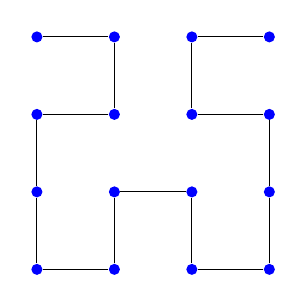
\begin{tikzpicture}[point/.style={circle,fill=blue,minimum size=4pt,inner sep=0pt}, node distance = 28pt]
        \node[point](0)                  {};
        \node[point](1)  [right of = 0]  {};
        \node[point](2)  [right of = 1]  {};
        \node[point](3)  [right of = 2]  {};
        \node[point](4)  [below of = 0]  {};
        \node[point](5)  [right of = 4]  {};
        \node[point](6)  [right of = 5]  {};        
        \node[point](7)  [right of = 6]  {};
        \node[point](8)  [below of = 4]  {};
        \node[point](9)  [right of = 8]  {};
        \node[point](10) [right of = 9]  {};
        \node[point](11) [right of = 10] {};
        \node[point](12) [below of = 8]  {};
        \node[point](13) [right of = 12] {};
        \node[point](14) [right of = 13] {};
        \node[point](15) [right of = 14] {};
        \path
          (0) edge node {} (1)
          (1) edge node {} (5)
          (2) edge node {} (3)
          (4) edge node {} (8)
          (5) edge node {} (4)
          (6) edge node {} (2)
          (7) edge node {} (6)
          (8) edge node {} (12)
          (9) edge node {} (10)
          (10) edge node {} (14)
          (11) edge node {} (7)
          (12) edge node {} (13)
          (13) edge node {} (9)
          (14) edge node {} (15) 
          (15) edge node {} (11)
          ;
      \end{tikzpicture}
    \end{minipage}
    \hfill
    \begin{minipage}{.3\textwidth}
      \begin{center}
        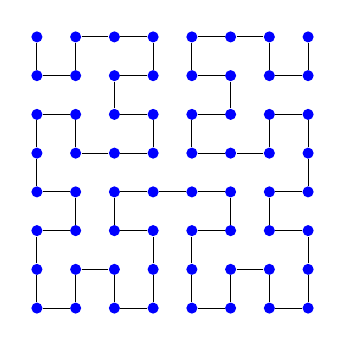
\begin{tikzpicture}[point/.style={circle,fill=blue,minimum size=4pt,inner sep=0pt}, node distance = 14pt]
          \node[point](0)                    {};
          \node[point](1)   [right of = 0]   {};
          \node[point](2)   [right of = 1]   {};
          \node[point](3)   [right of = 2]   {};
          \node[point](4)   [right of = 3]   {};
          \node[point](5)   [right of = 4]   {};
          \node[point](6)   [right of = 5]   {};
          \node[point](7)   [right of = 6]   {};
          \node[point](8)   [below of = 0]   {};
          \node[point](9)   [right of = 8]   {};
          \node[point](10)  [right of = 9]   {};
          \node[point](11)  [right of = 10]  {};
          \node[point](12)  [right of = 11]  {};
          \node[point](13)  [right of = 12]  {};
          \node[point](14)  [right of = 13]  {};
          \node[point](15)  [right of = 14]  {};
          \node[point](16)  [below of = 8]   {};
          \node[point](17)  [right of = 16]  {};
          \node[point](18)  [right of = 17]  {};
          \node[point](19)  [right of = 18]  {};
          \node[point](20)  [right of = 19]  {};
          \node[point](21)  [right of = 20]  {};
          \node[point](22)  [right of = 21]  {};
          \node[point](23)  [right of = 22]  {};
          \node[point](24)  [below of = 16]  {};
          \node[point](25)  [right of = 24]  {};
          \node[point](26)  [right of = 25]  {};
          \node[point](27)  [right of = 26]  {};
          \node[point](28)  [right of = 27]  {};
          \node[point](29)  [right of = 28]  {};
          \node[point](30)  [right of = 29]  {};
          \node[point](31)  [right of = 30]  {};
          \node[point](32)  [below of = 24]  {};
          \node[point](33)  [right of = 32]  {};
          \node[point](34)  [right of = 33]  {};
          \node[point](35)  [right of = 34]  {};
          \node[point](36)  [right of = 35]  {};
          \node[point](37)  [right of = 36]  {};
          \node[point](38)  [right of = 37]  {};
          \node[point](39)  [right of = 38]  {};
          \node[point](40)  [below of = 32]  {};
          \node[point](41)  [right of = 40]  {};
          \node[point](42)  [right of = 41]  {};
          \node[point](43)  [right of = 42]  {};
          \node[point](44)  [right of = 43]  {};
          \node[point](45)  [right of = 44]  {};
          \node[point](46)  [right of = 45]  {};
          \node[point](47)  [right of = 46]  {};
          \node[point](48)  [below of = 40]  {};
          \node[point](49)  [right of = 48]  {};
          \node[point](50)  [right of = 49]  {};
          \node[point](51)  [right of = 50]  {};
          \node[point](52)  [right of = 51]  {};
          \node[point](53)  [right of = 52]  {};
          \node[point](54)  [right of = 53]  {};
          \node[point](55)  [right of = 54]  {};
          \node[point](56)  [below of = 48]  {};
          \node[point](57)  [right of = 56]  {};
          \node[point](58)  [right of = 57]  {};
          \node[point](59)  [right of = 58]  {};
          \node[point](60)  [right of = 59]  {};
          \node[point](61)  [right of = 60]  {};
          \node[point](62)  [right of = 61]  {};
          \node[point](63)  [right of = 62]  {};
          \path
            (0) edge node {} (8)
            (8) edge node {} (9)
            (9) edge node {} (1)
            (1) edge node {} (2)
            (2) edge node {} (3)
            (3) edge node {} (11)
            (11) edge node {} (10)
            (10) edge node {} (18)
            (18) edge node {} (19)
            (19) edge node {} (27)
            (27) edge node {} (26)
            (26) edge node {} (25)
            (25) edge node {} (17)
            (17) edge node {} (16)
            (16) edge node {} (24)
            (24) edge node {} (32)
            (32) edge node {} (33)
            (33) edge node {} (41)
            (41) edge node {} (40)
            (40) edge node {} (48)
            (48) edge node {} (56)
            (56) edge node {} (57)
            (57) edge node {} (49)
            (49) edge node {} (50)
            (50) edge node {} (58)
            (58) edge node {} (59)
            (59) edge node {} (51)
            (51) edge node {} (43)
            (43) edge node {} (42)
            (42) edge node {} (34)
            (34) edge node {} (35)
            (35) edge node {} (36)
            (36) edge node {} (37)
            (37) edge node {} (45)
            (45) edge node {} (44)
            (44) edge node {} (52)
            (52) edge node {} (60)
            (60) edge node {} (61)
            (61) edge node {} (53)
            (53) edge node {} (54)
            (54) edge node {} (62)
            (62) edge node {} (63)
            (63) edge node {} (55)
            (55) edge node {} (47)
            (47) edge node {} (46)
            (46) edge node {} (38)
            (38) edge node {} (39)
            (39) edge node {} (31)
            (31) edge node {} (23)
            (23) edge node {} (22)
            (22) edge node {} (30)
            (30) edge node {} (29)
            (29) edge node {} (28)
            (28) edge node {} (20)
            (20) edge node {} (21)
            (21) edge node {} (13)
            (13) edge node {} (12)
            (12) edge node {} (4)
            (4) edge node {} (5)
            (5) edge node {} (6)
            (6) edge node {} (14)
            (14) edge node {} (15)
            (15) edge node {} (7)
            ;
        \end{tikzpicture}
      \end{center}
    \end{minipage}
  \end{center}
  \caption{The first three Hilbert curve iterations}
  \label{fig:hilbertiters}
\end{figure}

That is why the work \cite{cortesi11} used the more complex Hilbert space-filling curve.
The Hilbert curve passes through every pixel in a square exactly once in such a recursive pattern for which consecutive pixels always share one side.\cite{hilbert91}
Moreover, placing pixels in these specific ways ensures that the shorter sequences are expanded into multiple lines and aggregated into clusters which makes them more easily visible.
The curve covers a square with the side length of $2^i$ pixels (i.e., a total of $4^i$ pixels) where $i$ is the number of iterations.

The order in which the Hilbert curve goes through pixels in a 2D plane for each of the first three iterations can be seen in the figure \ref{fig:hilbertiters}.

However, when using the Hilbert curve, another problem arises.
There is no intuitive way to tell where the visualized sectors are located in the source image.

A middle ground between simple sweeping and the Hilbert curve would be the technique of block-sweeping I came up with.
Block-sweeping uses the sweeping method to fill up a square NxN pixels in size, then continues to another NxN pixel block and places these pixel blocks in the same way simple sweeping would place individual pixels.
This means that sweeping is just a version of block-sweeping, with pixel blocks of 1x1 pixels.
By employing this technique, most shorter sequences are still more pronounced by getting expanded into multiple lines, and the position of pixels in the image more closely resembles the sector position in the source image than in the Hilbert curve.
However, same as with sweeping, consecutive sectors are not always guaranteed to be right next to each other.

Figure \ref{fig:visorders} depicts the order in which the sweeping, 2x2 block sweeping, and 4x4 block sweeping methods visit pixels.
\begin{figure}
  \begin{center}
    \begin{minipage}{.3\textwidth}
    \begin{center}
      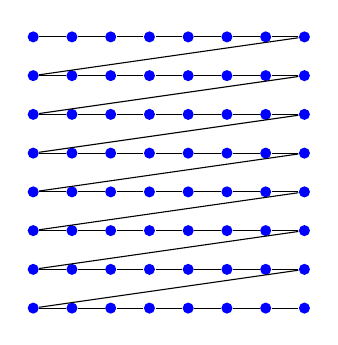
\begin{tikzpicture}[point/.style={circle,fill=blue,minimum size=4pt,inner sep=0pt}, node distance = 14pt]
          \node[point](0)                    {};
          \node[point](1)  [right of = 0]    {};
          \node[point](2)  [right of = 1]    {};
          \node[point](3)  [right of = 2]    {};
          \node[point](4)  [right of = 3]    {};
          \node[point](5)  [right of = 4]    {};
          \node[point](6)  [right of = 5]    {};
          \node[point](7)  [right of = 6]    {};
          \node[point](8)  [below of = 0]    {};
          \node[point](9)  [right of = 8]    {};
          \node[point](10)  [right of = 9]   {};
          \node[point](11)  [right of = 10]  {};
          \node[point](12)  [right of = 11]  {};
          \node[point](13)  [right of = 12]  {};
          \node[point](14)  [right of = 13]  {};
          \node[point](15)  [right of = 14]  {};
          \node[point](16)  [below of = 8]   {};
          \node[point](17)  [right of = 16]  {};
          \node[point](18)  [right of = 17]  {};
          \node[point](19)  [right of = 18]  {};
          \node[point](20)  [right of = 19]  {};
          \node[point](21)  [right of = 20]  {};
          \node[point](22)  [right of = 21]  {};
          \node[point](23)  [right of = 22]  {};
          \node[point](24)  [below of = 16]  {};
          \node[point](25)  [right of = 24]  {};
          \node[point](26)  [right of = 25]  {};
          \node[point](27)  [right of = 26]  {};
          \node[point](28)  [right of = 27]  {};
          \node[point](29)  [right of = 28]  {};
          \node[point](30)  [right of = 29]  {};
          \node[point](31)  [right of = 30]  {};
          \node[point](32)  [below of = 24]  {};
          \node[point](33)  [right of = 32]  {};
          \node[point](34)  [right of = 33]  {};
          \node[point](35)  [right of = 34]  {};
          \node[point](36)  [right of = 35]  {};
          \node[point](37)  [right of = 36]  {};
          \node[point](38)  [right of = 37]  {};
          \node[point](39)  [right of = 38]  {};
          \node[point](40)  [below of = 32]  {};
          \node[point](41)  [right of = 40]  {};
          \node[point](42)  [right of = 41]  {};
          \node[point](43)  [right of = 42]  {};
          \node[point](44)  [right of = 43]  {};
          \node[point](45)  [right of = 44]  {};
          \node[point](46)  [right of = 45]  {};
          \node[point](47)  [right of = 46]  {};
          \node[point](48)  [below of = 40]  {};
          \node[point](49)  [right of = 48]  {};
          \node[point](50)  [right of = 49]  {};
          \node[point](51)  [right of = 50]  {};
          \node[point](52)  [right of = 51]  {};
          \node[point](53)  [right of = 52]  {};
          \node[point](54)  [right of = 53]  {};
          \node[point](55)  [right of = 54]  {};
          \node[point](56)  [below of = 48]  {};
          \node[point](57)  [right of = 56]  {};
          \node[point](58)  [right of = 57]  {};
          \node[point](59)  [right of = 58]  {};
          \node[point](60)  [right of = 59]  {};
          \node[point](61)  [right of = 60]  {};
          \node[point](62)  [right of = 61]  {};
          \node[point](63)  [right of = 62]  {};
        \path
          (0) edge node {} (1)
          (1) edge node {} (2)
          (2) edge node {} (3)
          (3) edge node {} (4)
          (4) edge node {} (5)
          (5) edge node {} (6)
          (6) edge node {} (7)
          (7) edge node {} (8)
          (8) edge node {} (9)
          (9) edge node {} (10)
          (10) edge node {} (11)
          (11) edge node {} (12)
          (12) edge node {} (13)
          (13) edge node {} (14)
          (14) edge node {} (15)
          (15) edge node {} (16)
          (16) edge node {} (17)
          (17) edge node {} (18)
          (18) edge node {} (19)
          (19) edge node {} (20)
          (20) edge node {} (21)
          (21) edge node {} (22)
          (22) edge node {} (23)
          (23) edge node {} (24)
          (24) edge node {} (25)
          (25) edge node {} (26)
          (26) edge node {} (27)
          (27) edge node {} (28)
          (28) edge node {} (29)
          (29) edge node {} (30)
          (30) edge node {} (31)
          (31) edge node {} (32)
          (32) edge node {} (33)
          (33) edge node {} (34)
          (34) edge node {} (35)
          (35) edge node {} (36)
          (36) edge node {} (37)
          (37) edge node {} (38)
          (38) edge node {} (39)
          (39) edge node {} (40)
          (40) edge node {} (41)
          (41) edge node {} (42)
          (42) edge node {} (43)
          (43) edge node {} (44)
          (44) edge node {} (45)
          (45) edge node {} (46)
          (46) edge node {} (47)
          (47) edge node {} (48)
          (48) edge node {} (49)
          (49) edge node {} (50)
          (50) edge node {} (51)
          (51) edge node {} (52)
          (52) edge node {} (53)
          (53) edge node {} (54)
          (54) edge node {} (55)
          (55) edge node {} (56)
          (56) edge node {} (57)
          (57) edge node {} (58)
          (58) edge node {} (59)
          (59) edge node {} (60)
          (60) edge node {} (61)
          (61) edge node {} (62)
          (62) edge node {} (63)
          ;
      \end{tikzpicture}
      \end{center}
    \end{minipage}
    \hfill
    \begin{minipage}{.3\textwidth}
      \begin{center}
        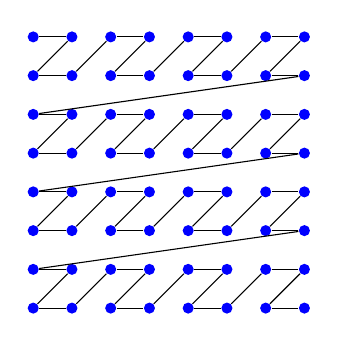
\begin{tikzpicture}[point/.style={circle,fill=blue,minimum size=4pt,inner sep=0pt}, node distance = 14pt]
          \node[point](0)                    {};
          \node[point](1)  [right of = 0]    {};
          \node[point](2)  [right of = 1]    {};
          \node[point](3)  [right of = 2]    {};
          \node[point](4)  [right of = 3]    {};
          \node[point](5)  [right of = 4]    {};
          \node[point](6)  [right of = 5]    {};
          \node[point](7)  [right of = 6]    {};
          \node[point](8)  [below of = 0]    {};
          \node[point](9)  [right of = 8]    {};
          \node[point](10)  [right of = 9]   {};
          \node[point](11)  [right of = 10]  {};
          \node[point](12)  [right of = 11]  {};
          \node[point](13)  [right of = 12]  {};
          \node[point](14)  [right of = 13]  {};
          \node[point](15)  [right of = 14]  {};
          \node[point](16)  [below of = 8]   {};
          \node[point](17)  [right of = 16]  {};
          \node[point](18)  [right of = 17]  {};
          \node[point](19)  [right of = 18]  {};
          \node[point](20)  [right of = 19]  {};
          \node[point](21)  [right of = 20]  {};
          \node[point](22)  [right of = 21]  {};
          \node[point](23)  [right of = 22]  {};
          \node[point](24)  [below of = 16]  {};
          \node[point](25)  [right of = 24]  {};
          \node[point](26)  [right of = 25]  {};
          \node[point](27)  [right of = 26]  {};
          \node[point](28)  [right of = 27]  {};
          \node[point](29)  [right of = 28]  {};
          \node[point](30)  [right of = 29]  {};
          \node[point](31)  [right of = 30]  {};
          \node[point](32)  [below of = 24]  {};
          \node[point](33)  [right of = 32]  {};
          \node[point](34)  [right of = 33]  {};
          \node[point](35)  [right of = 34]  {};
          \node[point](36)  [right of = 35]  {};
          \node[point](37)  [right of = 36]  {};
          \node[point](38)  [right of = 37]  {};
          \node[point](39)  [right of = 38]  {};
          \node[point](40)  [below of = 32]  {};
          \node[point](41)  [right of = 40]  {};
          \node[point](42)  [right of = 41]  {};
          \node[point](43)  [right of = 42]  {};
          \node[point](44)  [right of = 43]  {};
          \node[point](45)  [right of = 44]  {};
          \node[point](46)  [right of = 45]  {};
          \node[point](47)  [right of = 46]  {};
          \node[point](48)  [below of = 40]  {};
          \node[point](49)  [right of = 48]  {};
          \node[point](50)  [right of = 49]  {};
          \node[point](51)  [right of = 50]  {};
          \node[point](52)  [right of = 51]  {};
          \node[point](53)  [right of = 52]  {};
          \node[point](54)  [right of = 53]  {};
          \node[point](55)  [right of = 54]  {};
          \node[point](56)  [below of = 48]  {};
          \node[point](57)  [right of = 56]  {};
          \node[point](58)  [right of = 57]  {};
          \node[point](59)  [right of = 58]  {};
          \node[point](60)  [right of = 59]  {};
          \node[point](61)  [right of = 60]  {};
          \node[point](62)  [right of = 61]  {};
          \node[point](63)  [right of = 62]  {};
          \path
            (0) edge node {} (1)
            (1) edge node {} (8)
            (2) edge node {} (3)
            (3) edge node {} (10)
            (4) edge node {} (5)
            (5) edge node {} (12)
            (6) edge node {} (7)
            (7) edge node {} (14)
            (8) edge node {} (9)
            (9) edge node {} (2)
            (10) edge node {} (11)
            (11) edge node {} (4)
            (12) edge node {} (13)
            (13) edge node {} (6)
            (14) edge node {} (15)
            (15) edge node {} (16)
            (16) edge node {} (17)
            (17) edge node {} (24)
            (18) edge node {} (19)
            (19) edge node {} (26)
            (20) edge node {} (21)
            (21) edge node {} (28)
            (22) edge node {} (23)
            (23) edge node {} (30)
            (24) edge node {} (25)
            (25) edge node {} (18)
            (26) edge node {} (27)
            (27) edge node {} (20)
            (28) edge node {} (29)
            (29) edge node {} (22)
            (30) edge node {} (31)
            (31) edge node {} (32)
            (32) edge node {} (33)
            (33) edge node {} (40)
            (34) edge node {} (35)
            (35) edge node {} (42)
            (36) edge node {} (37)
            (37) edge node {} (44)
            (38) edge node {} (39)
            (39) edge node {} (46)
            (40) edge node {} (41)
            (41) edge node {} (34)
            (42) edge node {} (43)
            (43) edge node {} (36)
            (44) edge node {} (45)
            (45) edge node {} (38)
            (46) edge node {} (47)
            (47) edge node {} (48)
            (48) edge node {} (49)
            (49) edge node {} (56)
            (50) edge node {} (51)
            (51) edge node {} (58)
            (52) edge node {} (53)
            (53) edge node {} (60)
            (54) edge node {} (55)
            (55) edge node {} (62)
            (56) edge node {} (57)
            (57) edge node {} (50)
            (58) edge node {} (59)
            (59) edge node {} (52)
            (60) edge node {} (61)
            (61) edge node {} (54)
            (62) edge node {} (63)
            ;
        \end{tikzpicture}
      \end{center}
    \end{minipage}
    \hfill
    \begin{minipage}{.3\textwidth}
      \begin{center}
        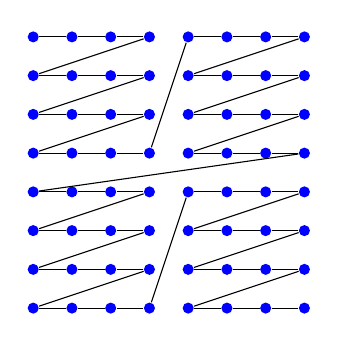
\begin{tikzpicture}[point/.style={circle,fill=blue,minimum size=4pt,inner sep=0pt}, node distance = 14pt]
          \node[point](0)                    {};
          \node[point](1)   [right of = 0]   {};
          \node[point](2)   [right of = 1]   {};
          \node[point](3)   [right of = 2]   {};
          \node[point](4)   [right of = 3]   {};
          \node[point](5)   [right of = 4]   {};
          \node[point](6)   [right of = 5]   {};
          \node[point](7)   [right of = 6]   {};
          \node[point](8)   [below of = 0]   {};
          \node[point](9)   [right of = 8]   {};
          \node[point](10)  [right of = 9]   {};
          \node[point](11)  [right of = 10]  {};
          \node[point](12)  [right of = 11]  {};
          \node[point](13)  [right of = 12]  {};
          \node[point](14)  [right of = 13]  {};
          \node[point](15)  [right of = 14]  {};
          \node[point](16)  [below of = 8]   {};
          \node[point](17)  [right of = 16]  {};
          \node[point](18)  [right of = 17]  {};
          \node[point](19)  [right of = 18]  {};
          \node[point](20)  [right of = 19]  {};
          \node[point](21)  [right of = 20]  {};
          \node[point](22)  [right of = 21]  {};
          \node[point](23)  [right of = 22]  {};
          \node[point](24)  [below of = 16]  {};
          \node[point](25)  [right of = 24]  {};
          \node[point](26)  [right of = 25]  {};
          \node[point](27)  [right of = 26]  {};
          \node[point](28)  [right of = 27]  {};
          \node[point](29)  [right of = 28]  {};
          \node[point](30)  [right of = 29]  {};
          \node[point](31)  [right of = 30]  {};
          \node[point](32)  [below of = 24]  {};
          \node[point](33)  [right of = 32]  {};
          \node[point](34)  [right of = 33]  {};
          \node[point](35)  [right of = 34]  {};
          \node[point](36)  [right of = 35]  {};
          \node[point](37)  [right of = 36]  {};
          \node[point](38)  [right of = 37]  {};
          \node[point](39)  [right of = 38]  {};
          \node[point](40)  [below of = 32]  {};
          \node[point](41)  [right of = 40]  {};
          \node[point](42)  [right of = 41]  {};
          \node[point](43)  [right of = 42]  {};
          \node[point](44)  [right of = 43]  {};
          \node[point](45)  [right of = 44]  {};
          \node[point](46)  [right of = 45]  {};
          \node[point](47)  [right of = 46]  {};
          \node[point](48)  [below of = 40]  {};
          \node[point](49)  [right of = 48]  {};
          \node[point](50)  [right of = 49]  {};
          \node[point](51)  [right of = 50]  {};
          \node[point](52)  [right of = 51]  {};
          \node[point](53)  [right of = 52]  {};
          \node[point](54)  [right of = 53]  {};
          \node[point](55)  [right of = 54]  {};
          \node[point](56)  [below of = 48]  {};
          \node[point](57)  [right of = 56]  {};
          \node[point](58)  [right of = 57]  {};
          \node[point](59)  [right of = 58]  {};
          \node[point](60)  [right of = 59]  {};
          \node[point](61)  [right of = 60]  {};
          \node[point](62)  [right of = 61]  {};
          \node[point](63)  [right of = 62]  {};
          \path
            (0) edge node {} (1)
            (1) edge node {} (2)
            (2) edge node {} (3)
            (3) edge node {} (8)
            (4) edge node {} (5)
            (5) edge node {} (6)
            (6) edge node {} (7)
            (7) edge node {} (12)
            (8) edge node {} (9)
            (9) edge node {} (10)
            (10) edge node {} (11)
            (11) edge node {} (16)
            (12) edge node {} (13)
            (13) edge node {} (14)
            (14) edge node {} (15)
            (15) edge node {} (20)
            (16) edge node {} (17)
            (17) edge node {} (18)
            (18) edge node {} (19)
            (19) edge node {} (24)
            (20) edge node {} (21)
            (21) edge node {} (22)
            (22) edge node {} (23)
            (23) edge node {} (28)
            (24) edge node {} (25)
            (25) edge node {} (26)
            (26) edge node {} (27)
            (27) edge node {} (4)
            (28) edge node {} (29)
            (29) edge node {} (30)
            (30) edge node {} (31)
            (31) edge node {} (32)
            (32) edge node {} (33)
            (33) edge node {} (34)
            (34) edge node {} (35)
            (35) edge node {} (40)
            (36) edge node {} (37)
            (37) edge node {} (38)
            (38) edge node {} (39)
            (39) edge node {} (44)
            (40) edge node {} (41)
            (41) edge node {} (42)
            (42) edge node {} (43)
            (43) edge node {} (48)
            (44) edge node {} (45)
            (45) edge node {} (46)
            (46) edge node {} (47)
            (47) edge node {} (52)
            (48) edge node {} (49)
            (49) edge node {} (50)
            (50) edge node {} (51)
            (51) edge node {} (56)
            (52) edge node {} (53)
            (53) edge node {} (54)
            (54) edge node {} (55)
            (55) edge node {} (60)
            (56) edge node {} (57)
            (57) edge node {} (58)
            (58) edge node {} (59)
            (59) edge node {} (36)
            (60) edge node {} (61)
            (61) edge node {} (62)
            (62) edge node {} (63)
            ;
        \end{tikzpicture}
      \end{center}
    \end{minipage}
  \end{center}
\caption{Sweeping, 2x2 block sweeping, and 4x4 block sweeping}
  \label{fig:visorders}
\end{figure}


\chapter{Used tools}
\label{chap:used-tools}
%\section{Programming language}
%When choosing the programming language, I was deciding mainly between the languages C and Python.

%While C is very efficient, this utility is not time-sensitive and has no real-time constraints.
%However, with the amount of data the utility is meant to process, its efficiency is very much desirable and can be the difference of having analysis take minutes instead of hours or even days.
%On the other hand, while not as efficient as C, Python provides many features, making the development and later extensibility much easier.
%Python also enables C integration, which may be helpful for implementing parts of code that are called repeatedly and require efficiency.

%Another point worthy of consideration was subjective -- my comfortability with the language.
%Even though I've taken multiple courses on C, I didn't feel confident enough to write this utility entirely in C because of my lack of experience working with external C libraries and writing programs with hundreds of lines that are also meant to be expanded on.

%Based on all of this, I chose Python.
% \section{Python}
% I chose Python 3\cite{python} based on several factors.
% The most significant factor was subjective -- my comfortability with the language.
% Based on this, my decision was mainly between C and Python.

% Another factor is efficiency.
% While this utility is not time-sensitive and has no real-time constraints, its efficiency is very desirable and can be the difference between analysis taking minutes and taking hours or even days.
% Here, C is the obvious winner.
% However, Python enables C integration\cite{python-extend}, which could be used to implement parts of code called tens of millions of times to speed up the utility's performance.

% Another consideration is the extensibility of the written code. One of my goals is to make the code as extensible as possible. While it is certainly possible to make easily extensible code in C, I did not feel confident enough to do it well.

% The next significant consideration was the availability of other tools and built-in libraries.
% Python provides a wide range of built-in modules, making programming easier like argparse\cite{argparse} and collections\cite{collections} while also having many other installable libraries, which are mostly platform-independent.
% C also has many helpful libraries, but many are platform-dependent and might not be available for other distributions.


This chapter describes the third-party python libraries the utility uses for both sector classification and visualization.

\section{Pillow}
\label{sec:pillow}

Pillow\cite{pillow} is an image manipulation library for Python, which is a fork of the discontinued library PIL\cite{pil}.
This library is used to visualize the analysis results.
Since the results should be visualized as an image, where each pixel represents a single disk sector, statistical visualization libraries like Matplotlib\cite{matplotlib}, seaborn\cite{waskom21}, or Gnuplot\cite{gnuplot} were not good choices as they were not created with this exact type of visualization in mind.
While they provide the means to create such visualizations, they are not as straightforward as the means provided by Pillow.
While Pillow offers many more features beyond the very basics needed, it still keeps the interface for drawing one pixel at a time very simple. 

\subsection{Image}
\label{ssec:image}

The module \texttt{PIL.Image} provides an essential toolkit for manipulating images.
Given the image mode (e.g., RGB or RGBA) and image size, function \texttt{Image.new} creates an instance of the \texttt{PIL.Image.Image} class.
The \texttt{Image} class stores the state of the resulting image and can be modified using its methods. 

The method \texttt{Image.putpixel} modifies the state of the Image object and changes the color of the pixel on the given coordinates to the given color.
\texttt{Image.save} tries to store the image on the provided path, and the method \texttt{Image.close} releases allocated memory. \cite{pillowimage}

\subsection{ImageDraw}
\label{ssec:imagedraw}

The module \texttt{PIL.ImageDraw} is used to modify the \texttt{Image} class from \texttt{PIL.Image} in more powerful ways than just changing single pixels.
Function \texttt{ImageDraw.Draw} creates a special context object for the given \texttt{Image} object, which can be used for further in-place modifications.
The class of the context object \texttt{ImageDraw.ImageDraw} provides a wide range of shape drawing methods.

The method \texttt{ImageDraw.rectangle}, allows for drawing a rectangle for provided coordinates and colors.
It is also possible to specify the width and color of the rectangle outline.
The method \texttt{ImageDraw.text} allows for writing a provided string in a font on the image.
Both of these methods can be used for drawing the image legend. \cite{pillowimagedraw}

\subsection{ImageFont}
\label{ssec-imagefont}

The \texttt{ImageFont} module is used to work with fonts with the Pillow library.
It provides the means to load any installed fonts by their name or from path using the function \texttt{ImageFont.truetype} or to load a fallback font in case no other font is found with the function \texttt{ImageFont.load\_default}.
\texttt{ImageFont.truetype} returns an instance of \texttt{ImageFont.FreeTypeFont} and \texttt{ImageFont.load\_default} returns \texttt{ImageFont.ImageFont}.
While neither of these classes is a subclass of the other, thanks to Python's duck typing can still be used interchangeably.
Both of these classes implement the method \texttt{ImageFont.getsize} for calculating the dimensions in pixels of the box occupied by provided text written in this font. \cite{pillowimagefont}


% Pillow\cite{pillow} is an image manipulation library for Python, which is a fork of the discontinued library PIL\cite{pil}.

% I am using this library to visualize the analysis results.
% Since I decided on the approach of visualizing the results as an image, where each pixel represents a single disk sector, statistical visualization libraries like Matplotlib\cite{matplotlib}, seaborn\cite{waskom21}, or Gnuplot\cite{gnuplot} were not good choices as they were not created with this exact type of visualization in mind and while they provide the means to create such visualizations, they are not as straightforward as the means provided by Pillow.
% While Pillow offers many more features beyond the very basics needed, it still keeps the interface for drawing one pixel at a time very simple.

\section{Scipy}
\label{sec:scipy}
SciPy\cite{scipy20} is a Python library for scientific computing.
This library is used to calculate the inverse cumulative distribution function for the chi-squared distribution.
SciPy provides a couple of different modules, but only one was used in the implementation.

\subsection{stats}
\label{ssec:stats}
The module \texttt{stats} can be used to calculate values of many discrete\cite{scipydescrete} or continuous\cite{scipycontinuous} statistical distributions, including the chi-squared distribution.
The module provides callable object \texttt{stats.chi2.ppf}, which calculates the percentile point function (inverse cumulative distribution function) for given probability and degrees of freedom.\cite{scipystatschi2}
The resulting value is then used as the threshold or limit for when the results of the chi-square statistic are significant and should therefore be marked as \emph{perfect random} or \emph{not random}.


% \section{Scipy}
% Scipy\cite{scipy20} is a Python library for scientific computing.
% I am using this library to calculate the boundaries of the chi-square statistic of random data with inverse cumulative distribution function for the chi-square distribution based on given degrees of freedom ($2^\text{number of bits of values} - 1$) and provided p-value boundaries.
% I am also using this library to calculate the Kolmogorov–Smirnov test.
%Since I intended to visualize the sectors using a bitmap, I needed a tool to generate these images.
%One option was to use libraries and utilities like matplotlib\cite{matplotlib} or gnuplot\cite{gnuplot}.

%Both the Python package matplotlib and the gnuplot utility provide the means to generate different graphs, charts, or diagrams.
%Both can generate images with one pixel per data point. A significant advantage of these plotting utilities is the ability to choose one of the premade colormaps for visualizing different entropies of sectors.
%However, the visualized data is not only from a single range of entropy, and the color should be dependent on other factors like the sector patterns.
%This is certainly possible to implement, but it might be non-trivial.
%Another advantage is that the color descriptions are easily insertable with automatic centering.

%Another option is to use an image manipulation library.
%The advantage of this approach is the straightforward way to have complete control over the resulting image.
%The disadvantage is the need to implement the color descriptions and color mapping myself.
%Since the implementation of color mapping is required either way and color description is not that hard to implement, I chose this option.

%The library I chose for image manipulation is the Pillow library\cite{pillow}, which provides a simple image manipulation interface
% \chapter{Entropy calculation}
% \chapter{Ways of visualization}.
\chapter{Implementation}
\label{chap:implementation}
This chapter focuses on the individual parts of the implementation.
%...rest of the description of the chapter... % TODO

The utility reads the provided disk image in blocks of the provided block size, analyzes the read data, and passes the results alongside information about the position of the read block to the visualization class.

\section{Analysis}
\label{sec:analysis2}
The utility provides several analysis methods.
These methods are each implemented as a class.
Each analysis class implements a \texttt{calc} method, which analyzes the provided buffer and returns the results.
The results take the form of a tuple and contain: detected randomness from the range $\langle0,1\rangle$, result flag, and a possible result argument (used to pass the single-byte patterns if found).

\subsection{Entropy}
\label{ssec:entropy}

The provided buffer's normalized Shannon's entropy can be calculated using the formula \eqref{eq:norm-entropy}.
However, since $P(x_i) = \frac{c_i}{s}$ where $c_i$ is the number of times the value $i$ was in the buffer and $s$ is the unchanging sector size, the formula can be simplified to

\begin{equation}
 -\frac{1}{8s}\sum_{i=0}^{255}(c_i * \log_2(c_i)) + \log_2(s)
 \label{eq:impl-entropy}
\end{equation}

The counts $c_i$ are calculated using \texttt{Counter} from the \texttt{collections} module\cite{collections}.
The fact that the \texttt{Counter} object only iterates over nonzero counts does not matter.
By the entropy definition, the impossible results should not affect it.

However, Shannon's entropy is not a statistical test, and its results are not used to distinguish between random and not random.
Therefore there are no levels of significance, and the analysis result is just a number from the range 0-1.
While this analysis does not help recognize random from non-random data at a glance, it can illustrate whether sectors with similar entropy (and therefore with similar file contents) are stored next to each other. 

Image generated with Shannon's entropy can be found in the figure \ref{fig:impl-shannon}.
The darker the shadow of red, the higher the detected entropy of the sector represented by the pixel.

\begin{figure}
    \centering
    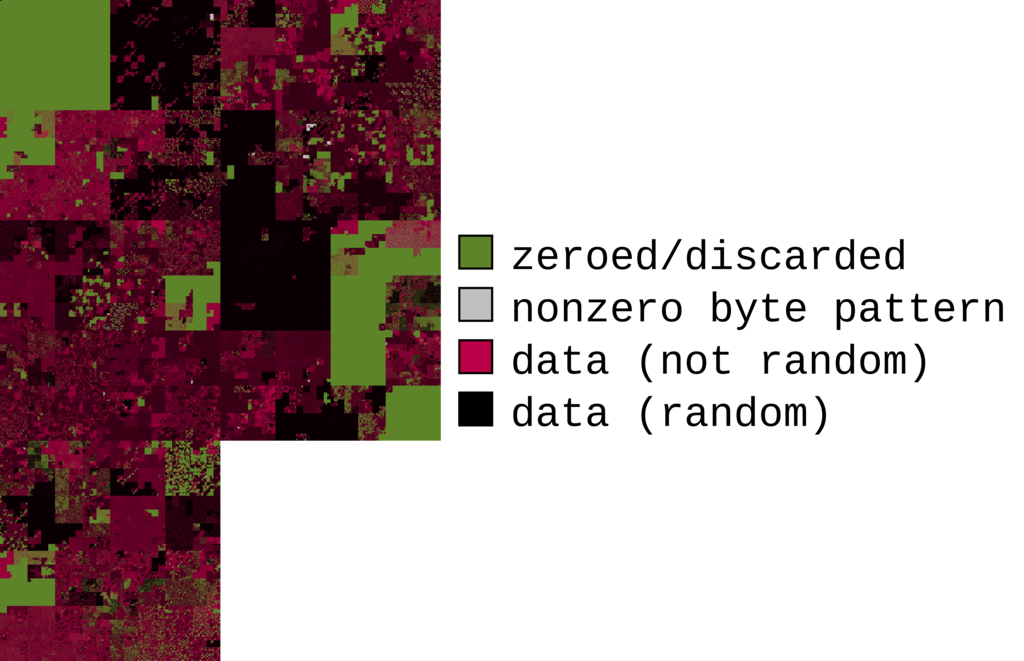
\includegraphics[width=\textwidth,interpolate=false]{ubnt-unencrypted-shannon-hilbert-asalor.png}
    \caption{Image generated with Shannon's entropy analysis and \texttt{asalor} palette from the same disk image as figure \ref{fig:veracrypt-without}}
    \label{fig:impl-shannon}
\end{figure}

\subsection{Chi-square}
\label{ssec:chi2}

The implementation includes multiple options for analysis by chi-square test.
Each option takes $n$ consecutive bits and treats them as a separate number.
If the sector size is not a multiple of $n$, the remaining bits are ignored.

The chi-square statistic can be calculated using the formula mentioned in the subsubsection \ref{sss:chi2-test}.
As the numbers should be from the uniform distribution and the expected count for each value should be the same, the formula can be modified to
$$\frac{1}{E}\sum_{i = 0}^{2^n - 1}((X_i - E)^2)$$
where $E$ is the expected count of each number and can be calculated using 
$$E = \frac{\lfloor\frac{8s}{n}\rfloor}{2^n}$$
where $s$ is the sector size in bytes.

Each option, while easily generalizable, is implemented separately due to possible speed improvements. 
(i.e., there is no need for reading a byte bit per bit and then merging the bits into an eight-bit number again; however, for $n = 3$, there is no such easy workaround)
\texttt{chi2-8} simply counts each byte value, \texttt{chi2-4} separates the byte values into halves using the python bitwise \texttt{\&} and \texttt{>{>}} operators, \texttt{chi2-3} goes through each byte bit-by-bit, and \texttt{chi2-1} uses the \texttt{int.bit\_count method} to get the number of bits set to 1 in the byte value.

Each method first calculates the expected count of each value.
If this value is less than 5, a warning about possible issues with precision\cite{knuth81} is printed.
This, however, occurs only for the combination of chi2-8 analysis and the sector size of 512 bytes (or lower, but 512 is the smallest commonly used sector size).
Then the method precalculates limits for the chi-square statistic, for which the sector is marked as \emph{perfect random}, \emph{random}, or \emph{not random}.
Then for each sector, its statistic is compared to these limits, and a matching output flag is selected.
All methods also check for single-byte patterns. The most common ones (i.e., \texttt{0x00} and \texttt{0xFF}) are always checked.
However, all other single-byte patterns are checked only by \texttt{chi2-8} and \texttt{chi2-4}.
These two implementations were already counting the number of bytes, and this check could be done with a minimal additional performance penalty.
Finding the other single-byte patterns is not essential as they are not likely to be contained unless they are part of an unencrypted stored file, which will almost always be marked as \emph{not random} by the analysis.
The only exception is with \texttt{chi2-1} for the seventy byte patterns, which contain an equal number of zeroes and ones, in which case the sector will be marked as \emph{perfect random}.

\section{Output and visualization}
\label{sec:output-and-visualization}

Each output method is implemented in the form of a class.
Each output class should implement the following three methods.
\begin{itemize}
    \item Method \texttt{output} for taking the analysis output and storing it.
    \item Method \texttt{error} to be run in case of an error to display it.
    \item Method \texttt{exit}, which is run before the program terminates to close any open data streams and save stored data into files.
\end{itemize}
Each output class can have an attribute \texttt{default\_parameters}, which is a mapping of a parameter name to \texttt{Parameter} dataclass, which stores the type of the parameter, default value, help string, and can also store string description of the default value and list of available options.

\subsection{Text output}
\label{ssec:text-output}

The utility, while being primarily intended for visualization, also implements two methods for text output.

The first one is \texttt{sample-output}, which just formats the analysis output of each sector on a seperate line as follows: <sector number> (<sector offset>) - <randomness>, <result flag> (pattern of: <single-byte pattern if present>)

The second method, \texttt{csv}, outputs the analysis result as a CSV file.
The script \texttt{from\_csv.py} can later use this CSV file to generate a visualization using the other output methods without analyzing the disk image again.

\subsection{Image output}
\label{ssec:image-output}

The result of all Image output methods is a bitmap, where each pixel represents the result of an analysis of one sector.
The image is created using the Pillow library.

Using the command line arguments, the user can change the image's color palette, background color, and legend text color.
When specifying the background color but not the text color, the text color is determined automatically using the contrast ratio and the relative luminance in accordance with W3 guidelines.\cite{w3guidelines}

Since the image needs to fit all of the sectors and the number of sectors can vary between different disk images, it is essential to have varying proportions of the output images.

The utility also provides means for generating the images using multiple color palettes.
The four implemented are \texttt{sample}, \texttt{asalor}, \texttt{rg}, and \texttt{photocopy-safe} palettes.
The \texttt{asalor} color palette is the one used in Milan Broz's blog\cite{broz11}.
The colors for palettes rg and photocopy-safe were taken from colorbrewer2.org \cite{brewer02}.
The \texttt{photocopy-safe} palette can be seen in the figure \ref{fig:impl-visualizations}.

The utility draws the color legend for all image output methods by default.

The images in figure \ref{fig:impl-visualizations} were generated from 16GiB disk image of modified Debian system with whole system encryption taken from the study materials of the course FI:PV204\footnote{\url{https://is.muni.cz/auth/el/fi/jaro2019/PV204/um/seminars/08_diskencryption/pv204_fde.zip}}.

\subsection{Sweeping and block sweeping}
\label{ssec:sweeping-and-block-sweeping}

The user can set both the image width and sweeping block size.
When both are provided, it is only checked that width is a multiple of sweeping block size.
When only width is provided, the smallest divisor of width larger or equal to 32 but smaller than square root of width is set as the sweeping block size.
If no such number exists largest divisor of width smaller than 32 is used.
The utility tries to form a rectangle closest to a square if the width is not defined.
In this case, the sweeping block size is set to 32 if not specified.

Sweeping is a special case of block sweeping with the sweeping block size set to 1.

Images generated using the sweeping and sweeping blocks method can be found in the figures \ref{fig:impl-sweeping} and \ref{fig:impl-sweeping-blocks}.

\subsection{Hilbert curve}
\label{ssec:hilbert-curve}

For the Hilbert curve, the image size can only be determined automatically.
The smallest single curve which would fit all the sectors needs to have precisely $i = \lceil\log_4(\text{number of sectors})\rceil$ iterations.
However, it is possible to put multiple Hilbert curves under each other and chain them together.
Therefore the implementation first checks whether up to three smaller curves (i.e., curves with $i - 1$ iterations) could fit all the sectors.
If that is the case, width is set to $2^{i - 1}$ and height to the needed number of curves in half-curve-width increments.
Otherwise, the calculated number of iterations is used.
And therefore, the height and width are the same and equal to $2^i$.

The algorithm used for transforming sector sequence numbers into x and y coordinates from the Hilbert curve has been adapted from the C implementation in \cite{wikihilbert}.
The C implementation from \cite{wikihilbert} is a special case of the algorithm from \cite{skilling04} adapted to use two dimensions and distance from the start rather than a transposed array of bits of the distance.


In order to chain multiple Hilbert curves under each other and still keep the locality-preserving properties, the curves portrayed in the figure \ref{fig:hilbertiters} need to be mirrored along their top-left to bottom-right diagonals.
This can be simply achieved by swapping the x and y coordinates.


\begin{figure}
    \centering
    \begin{subfigure}[t]{.45\textwidth}
        \centering
        
\includegraphics[width=\textwidth,interpolate=false]{pv204_fde-chi2-4-sweeping.png}
        \caption{Sweeping}
        \label{fig:impl-sweeping}
    \end{subfigure}
    \hfill
    \begin{subfigure}[t]{.45\textwidth}
        \centering
        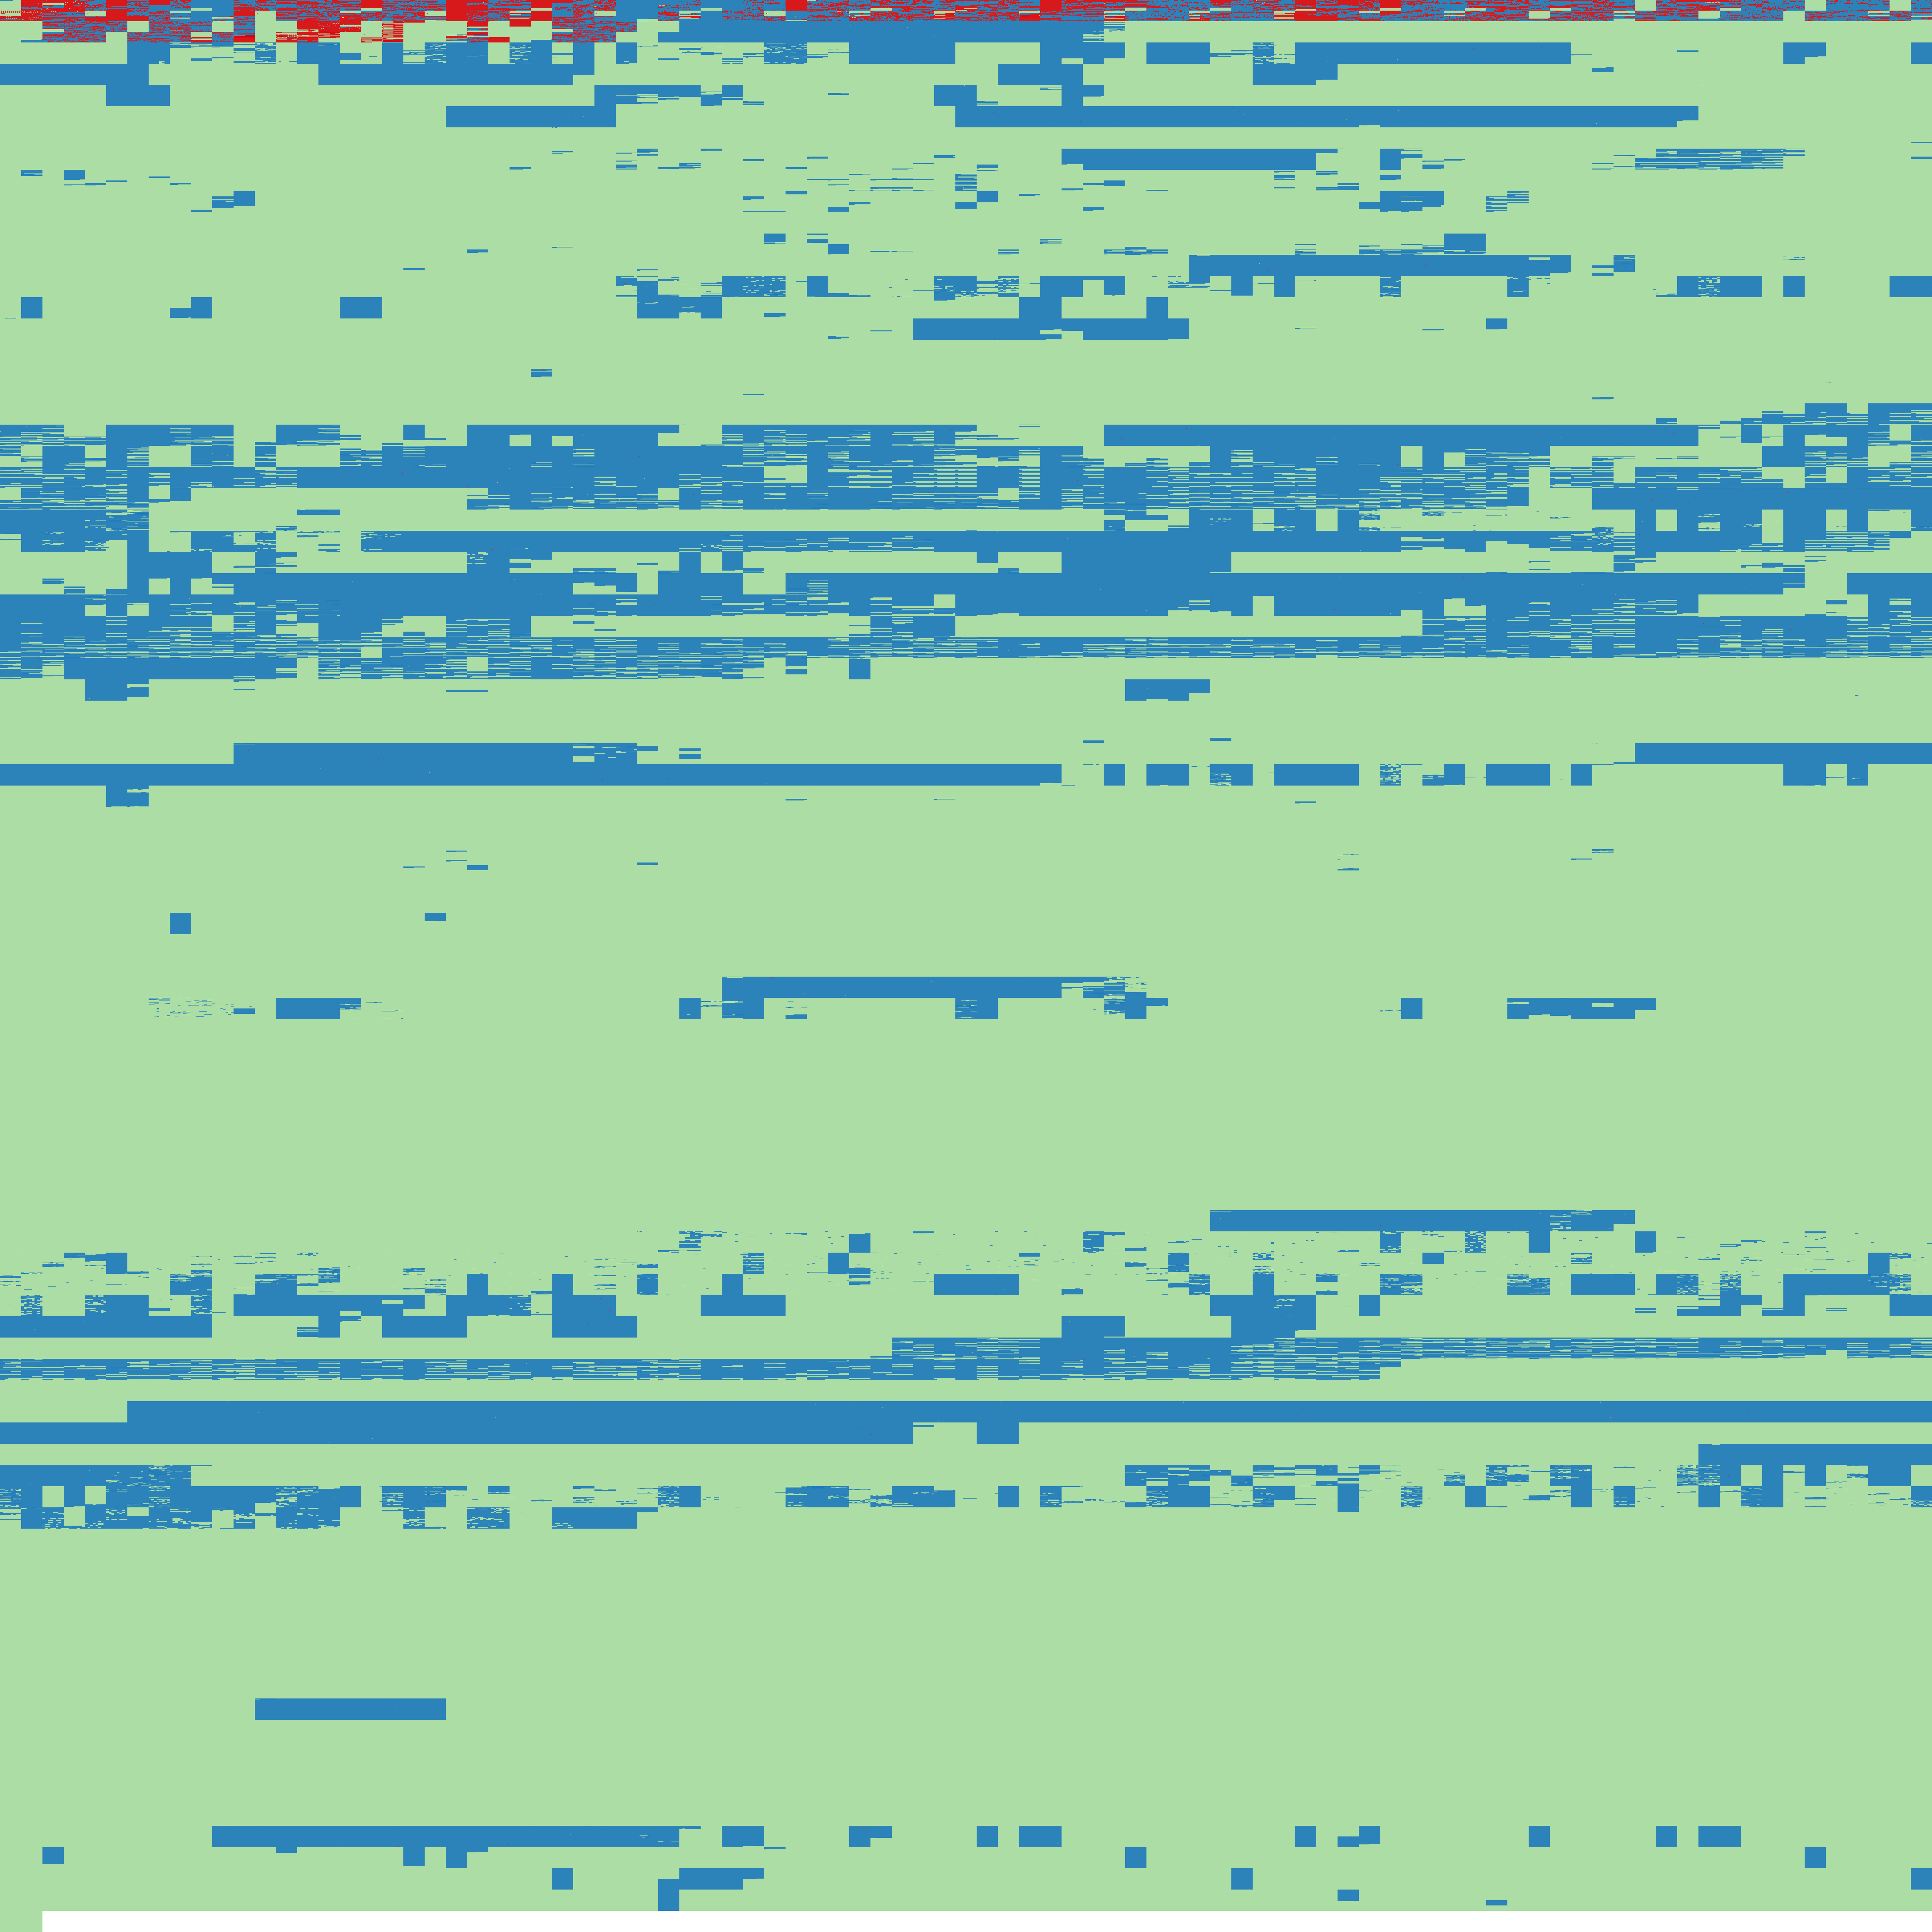
\includegraphics[width=\textwidth,interpolate=false]{pv204_fde-chi2-4-sweeping-blocks.png}
        \caption{Sweeping blocks}
        \label{fig:impl-sweeping-blocks}
    \end{subfigure}
    % \hfill
    \begin{subfigure}[t]{.6\textwidth}
        \centering
        \includegraphics[width=\textwidth,interpolate=false]{pv204_fde-chi2-4-hilbert.png}
        \caption{Hilbert curve with legend}
        \label{fig:impl-hilbert-curve}
    \end{subfigure}
    \caption{A 16GiB disk image visualized using all three image visualization methods}
    \label{fig:impl-visualizations}
\end{figure}

\chapter{Results}
\label{chap:results}
This chapter showcases examples of what the utility could be used for.

All images were generated with the utility with its parameters set as follows:
\begin{itemize}
  \item sector size of 512B
  \item chi2-4 analysis method
  \item the significance level of 0.0002
  \item photocopy-safe palette
\end{itemize}

The output method changes from figure to figure and is always mentioned in the figure caption.

\section{Used color palette}
\label{sec:used-color-palette}

All utility-generated images in this chapter were generated using the \texttt{photocopy-safe} palette.
This palette is specifically designed to be still readable after conversion to grayscale.
The \texttt{photocopy-safe} palette represents by light-green color the sectors that the analysis has marked as containing only zeroes.
Pixels of yellow color represent sectors that only contain a single-byte pattern, which is not of byte 0.
Unlike other implemented palettes, its shade does not represent the repeated byte value and is constant for each non-zero repeated byte value.
Orange represents sectors marked as \emph{perfect random}.

And finally, all other sectors are marked by shades between blue and red.
This shade depends on the detected randomness by the analysis.
For statistic-test-based analysis, the results are purely binary.
By blue are represented sectors marked as \emph{random}, and red represents sectors marked as \emph{not random}.

For the analysis using Shannon's entropy, the shade of purple represents the entropy detected.
The bluer the sector is, the higher its entropy, and the redder sector is, the lower its entropy.
Pictures generated using Shannon's entropy analysis cannot contain orange as it cannot mark sectors as \emph{perfect random}.

As all images in this chapter were analyzed using the \texttt{chi2-4} analysis method, the colors marking the randomness are only blue or red.

The legend of the used palette can be found in the figure \ref{fig:legend}.

% All utility-generated images in this chapter were generated using the \texttt{sample-palette}.
% The \texttt{sample-palette} represents by blue color the sectors that the analysis has marked as containing only zeroes.
% Pixels of green color represent sectors that only contain a single-byte pattern, which is not of byte \texttt{x00}.
% The shade of green represents the repeated byte value (i.e., the brightest green \texttt{xFF} and dimmest green \texttt{x01}).
% Red represents sectors marked as \emph{perfect random}. 

% And finally, by magenta are marked all the remaining sectors. The shade of magenta depends on the detected randomness by the analysis. For analysis using Shannon's entropy, the resulting shades of magenta range from black for the lowest but larger than 0 entropy to the brightest magenta (i.e., \texttt{\#FF00FF} in hex color representation) for the highest entropy. 

% On the other hand, the chi2 analysis variants only produce two shades of magenta. The lighter shade represents sectors marked as random the darker shade marks all sectors that do not contain a single-byte pattern and are marked as not random. Furthermore, red pixels are only contained in the images analyzed through the chi2 analysis variants as Shannon's entropy analysis cannot mark sectors as \emph{perfect random}.

Legend is not included in every image for space-saving reasons but can be found in the figure \ref{fig:legend}.

\begin{figure}[H]
  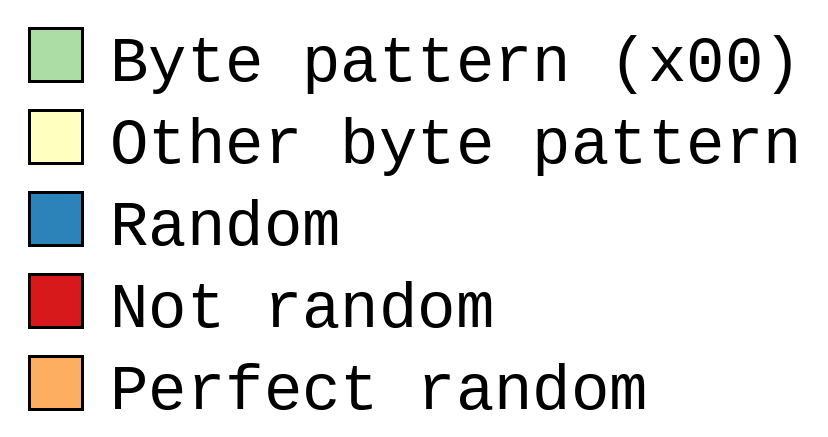
\includegraphics[width=.45\textwidth,interpolate=true]{legend.png}
  \caption{Legend for images generated using \texttt{sample-palette}}
  \label{fig:legend}
\end{figure}

\section{TRIM}
\label{sec:trim}

In order to show how TRIM affects the data stored on the disk and how the utility visualizes it crpytsetup 2.4.3 was used. 
First, a plain dm-crypt mapping with allowed discards to a 2GiB file was created.
Then through the mapping, a file system was created into which an unpacked Linux kernel 5.16.9 was copied.
Then, all the files in the largest directory, \texttt{drivers}, were deleted.
After deleting the files, a copy of the image was taken.
Generated images of analyses of these copies can be found in figures \ref{fig:trim-ext4-no-trim} and \ref{fig:trim-xfs-no-trim}.
These copies were then compared to the resulting image after calling \texttt{fstrim} on the mounted mapper, which discarded all unused sectors.
Images generated from images with discarded sectors can be found in figures \ref{fig:trim-ext4-trim} and \ref{fig:trim-xfs-trim}.

\begin{figure}
  \centering
  \begin{subfigure}[t]{0.45\textwidth}
    \centering
    
\includegraphics[width=\textwidth,interpolate=false]{test-ext4-no-trim-chi2-4-sweeping.png}
    \caption{Encrypted ext4 without TRIM}
    \label{fig:trim-ext4-no-trim}
  \end{subfigure}
  \hfill
  \begin{subfigure}[t]{0.45\textwidth}
    \centering
    
\includegraphics[width=\textwidth,interpolate=false]{test-ext4-chi2-4-sweeping.png}
    \caption{Encrypted ext4 with TRIM}
    \label{fig:trim-ext4-trim}
  \end{subfigure}
  \begin{subfigure}[b]{0.45\textwidth}
    \centering
    
\includegraphics[width=\textwidth,interpolate=false]{test-xfs-no-trim-chi2-4-sweeping.png}
    \caption{Encrypted xfs without TRIM}
    \label{fig:trim-xfs-no-trim}
  \end{subfigure}
  \hfill
  \begin{subfigure}[b]{0.45\textwidth}
    \centering
    
\includegraphics[width=\textwidth,interpolate=false]{test-xfs-chi2-4-sweeping.png}
    \caption{Encrypted xfs with TRIM}
    \label{fig:trim-xfs-trim}
  \end{subfigure}
  \begin{subfigure}[b]{0.45\textwidth}
    \centering
    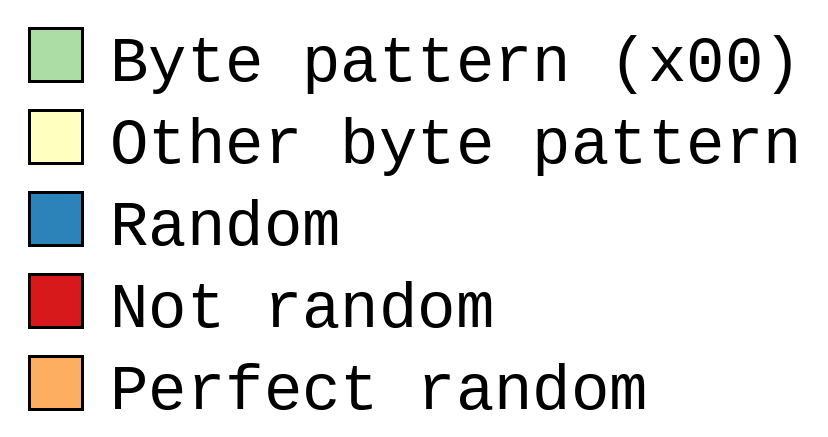
\includegraphics[width=\textwidth]{legend.png}
    \caption{Legend}
    \label{fig:trim-legend1}
  \end{subfigure}
  \caption{Comparison of encrypted filesystems with and without TRIM generated by the \texttt{sweeping} output method}
  \label{fig:trim-comparison}
\end{figure}

At first glance, one can see the difference.
The sectors marked by green are the ones that were discarded, and it can be clearly seen how many sectors the data actually takes up and where precisely the encrypted data is stored.

This need not necessarily be a huge security risk; however, in cases when it is vital not to show such information, it is good to be wary of such drawbacks of allowing trim commands.

Note that the blue is not solid, and one can, after a closer inspection, occasionally see sectors marked by orange or red, which are the result of sectors randomly having the p-value of its chi-square statistic outside of the bounds defined by the default significance value of 0.0002.
The number of these outlier pixels can be decreased by decreasing the significance level with the cost of decreasing the number of truly non-random sectors correctly identified as non-random.
A closeup of these pixels can be seen in the figure \ref{fig:trim-zoomed}.

\begin{figure}
    \centering
    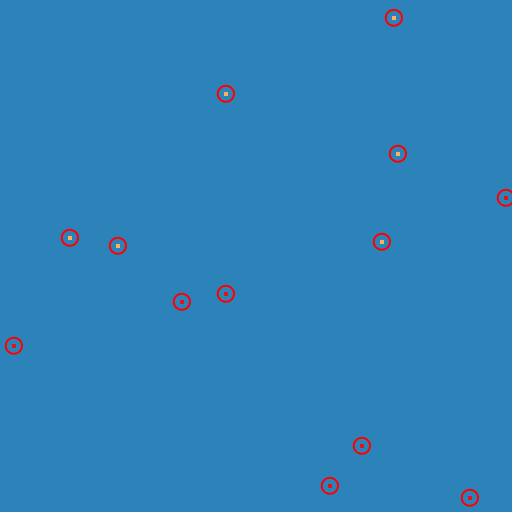
\includegraphics[width=.95\textwidth,interpolate=false]{test-ext4-no-trim-chi2-4-sweeping-zoomed.png}
    \caption{Zoomed in figure \ref{fig:trim-ext4-no-trim} with sectors marked as \emph{not random} or \emph{perfect random} highlighted with red circles}
    \label{fig:trim-zoomed}
\end{figure}

\section{Flawed encryption detection}
\label{sec:flawed-encryption}

For illustration, a fresh Canonical Ubuntu 20.04\cite{ubuntu} installation with the ext4 filesystem was created without encryption.
Then a file of the size of one gigabyte containing only a repeating word 'test' was written.
After analyzing the 10 GiB disk image using the analysis method of \texttt{chi2-4} and visualizing it using the Hilbert curve visualization method, the image in the figure \ref{fig:bad-enc-unenc} was produced.
On the generated image, one can distinctly see many areas of sectors of zeroes and also areas of sectors of unencrypted data.

Then OpenSSL 1.1.1n\cite{openssl} was used to encrypt the entire disk image with 128-bit AES in ECB mode.
Using the same analysis and visualization methods on the encrypted disk image as on the unencrypted variant, the utility generated the image in the figure \ref{fig:bad-enc-enc}.
On the resulting image are evidently visible areas of detected unencrypted sectors.
These are mostly the result of encrypting sectors of zeroes and, if the flawed encryption method were to be used and sector discarding was to be enabled, would most likely be trimmed and visible as zeroed regardless.
However, many areas that previously contained more complex data also remained marked as \emph{not random}.
Therefore not only would trimmed sectors be affected, but this effect can also occur in sectors storing actual data.

\begin{figure}
    \centering
    \begin{subfigure}[t]{.45\textwidth}
        \centering
        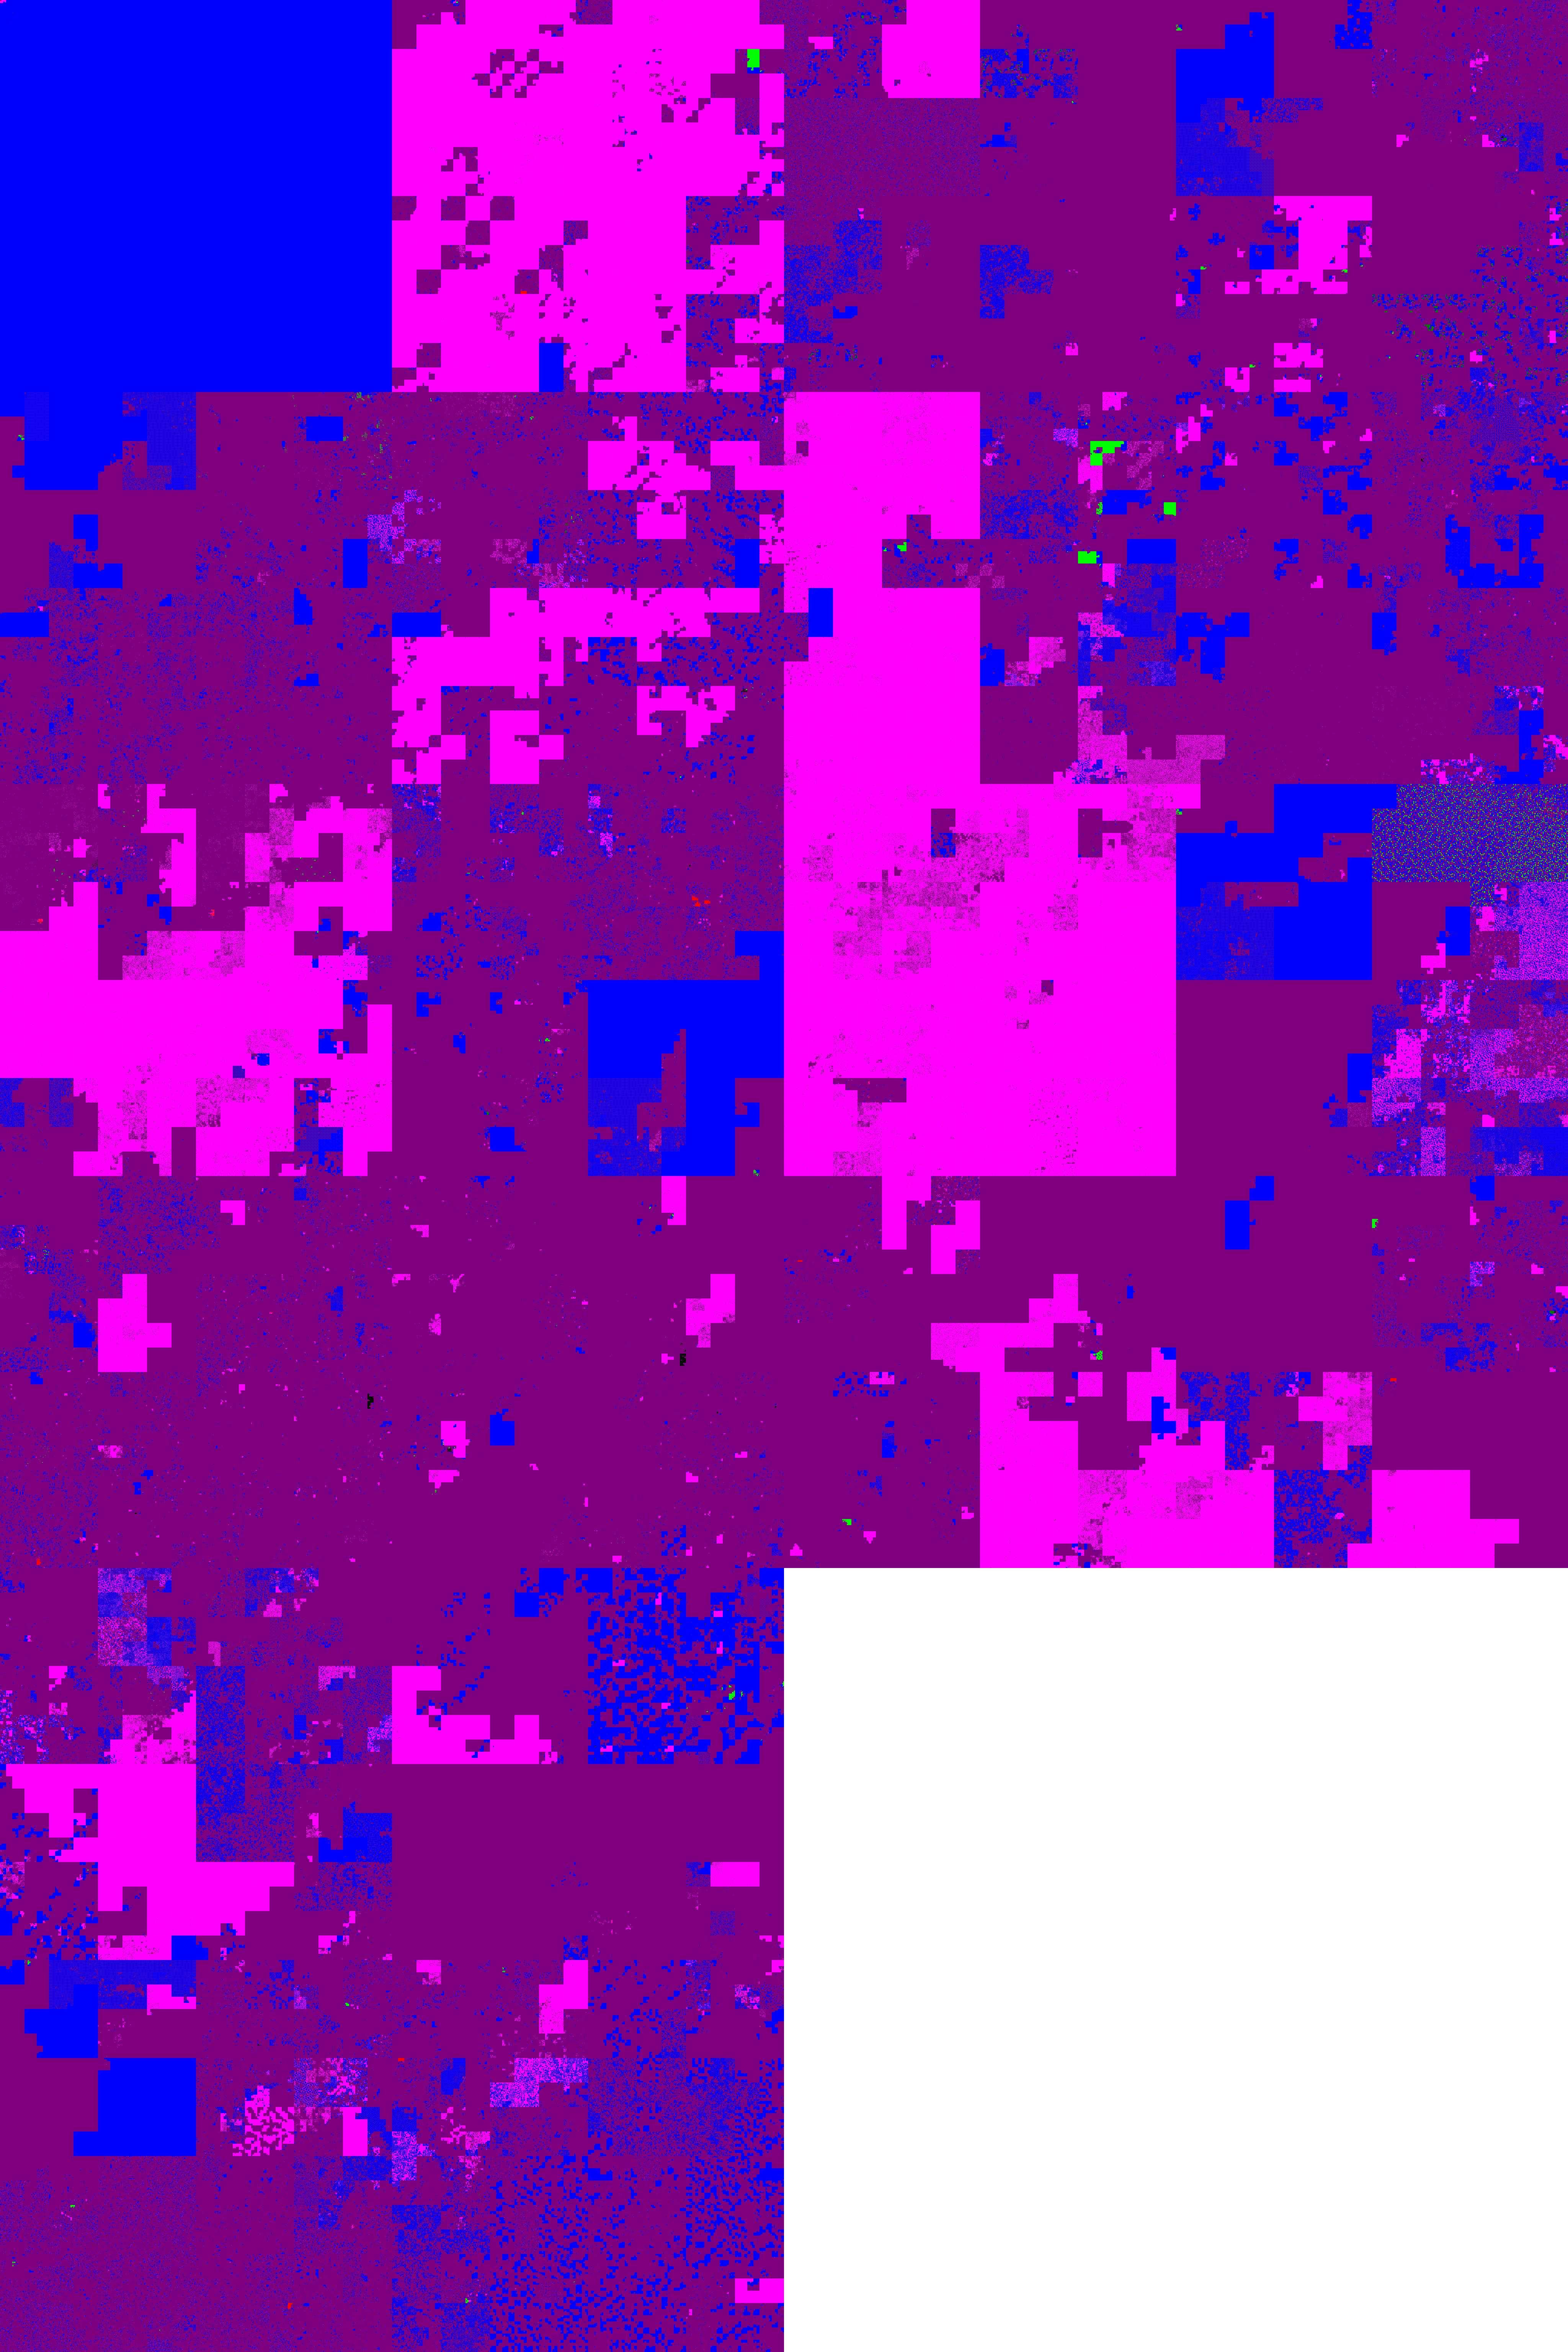
\includegraphics[width=\textwidth,interpolate=false]{ubnt-unencrypted-test-chi2-4-hilbert.png}
        \caption{Unencrypted}
        \label{fig:bad-enc-unenc}
    \end{subfigure}
    \hfill
    \begin{subfigure}[t]{.45\textwidth}
        \centering
        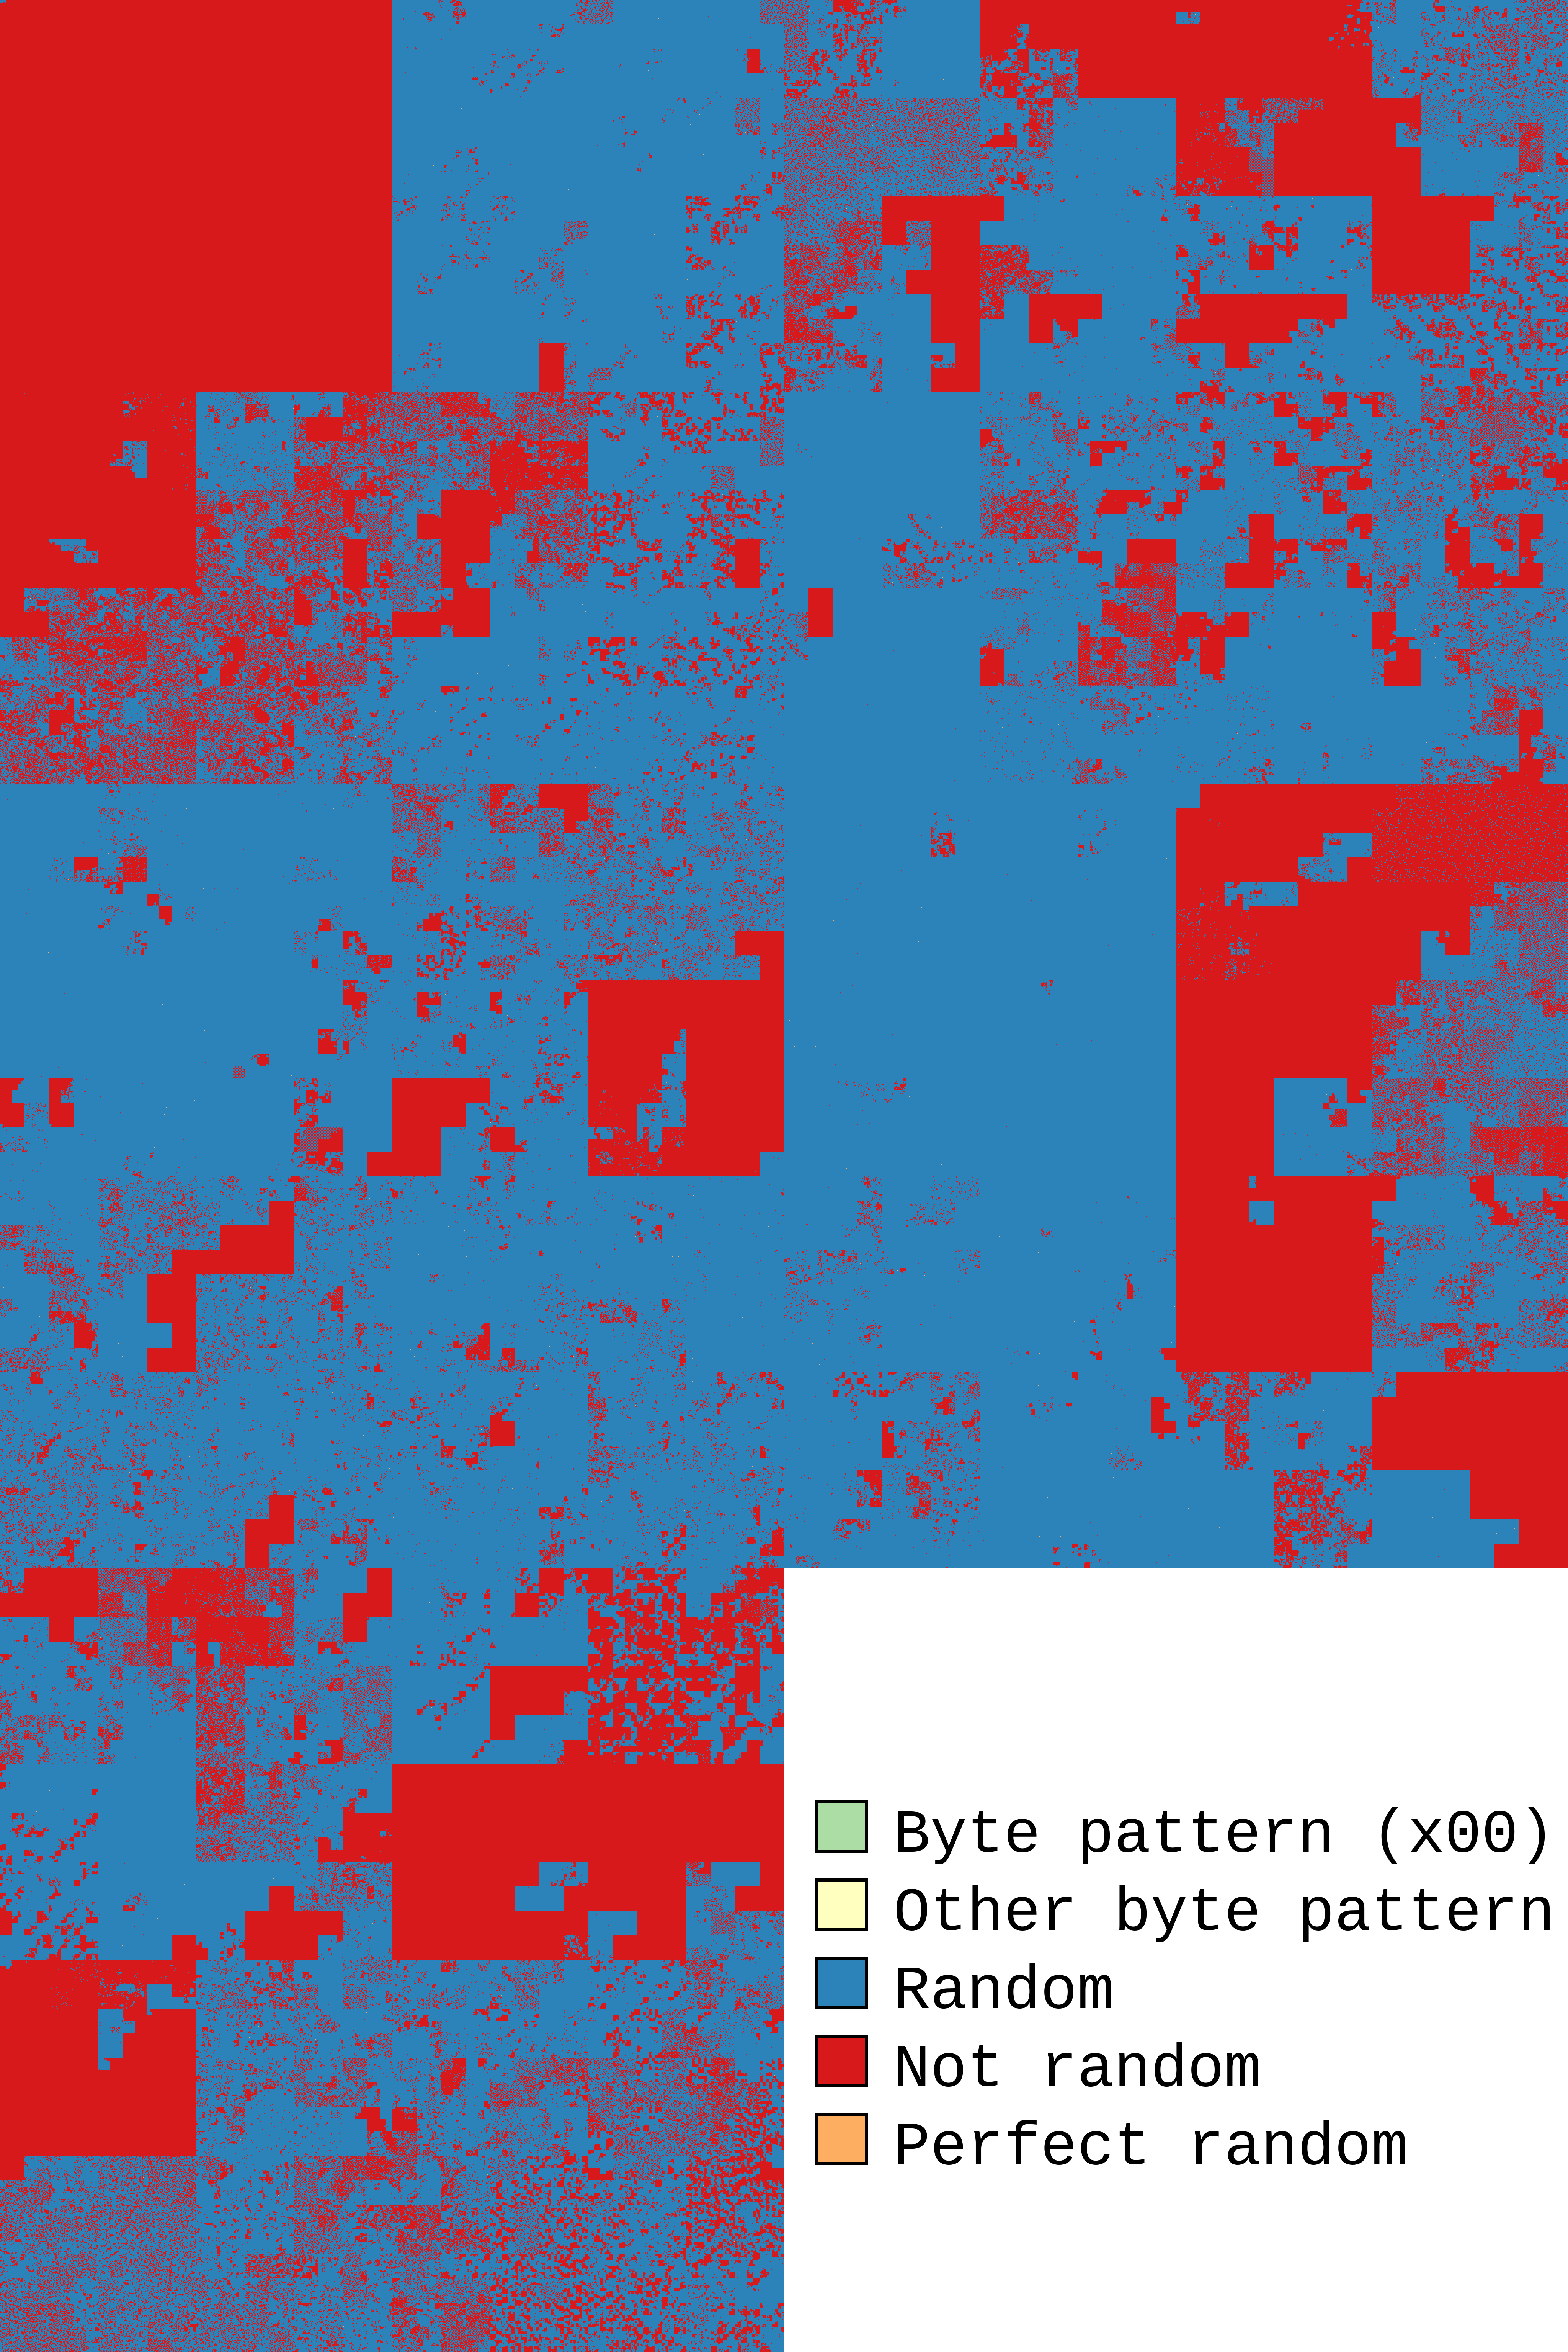
\includegraphics[width=\textwidth,interpolate=false]{ubnt-test-aes-128-ecb-chi2-4-hilbert-legend.png}
        \caption{Encrypted with 128-bit AES in ECB mode}
        \label{fig:bad-enc-enc}
     \end{subfigure}
    \caption{10GiB disk images visualized using \texttt{chi2-4} analysis method and hilbert curve}
    \label{fig:bad-enc-fig}
\end{figure}

This is caused by the ECB mode's property of encrypting every same block of bytes to the same encrypted block of bytes.
Since the sectors contain multiple sectors of the same blocks, the \texttt{chi2-4} analysis method picks up on it and marks the sector as \emph{not random}.

\section{Visualizing encrypted and unencrypted parts of a disk}
\label{sec:visualizing-encrypted-and-unencrypted-parts-of-a-disk}

For each of the following examples, a different disk image was used.

\subsection{BitLocker full volume encryption}
\label{ssec:bitlocker-full-volume-encryption}

For this example, a clean Windows 10 installation was created on a 50GiB virtual drive through Oracle VM VirtualBox.
First, a raw copy of the disk image was taken using VBoxManage.
Then, using the BitLocker user interface, full disk encryption was set up, after which another raw copy was taken.
Then the images in the figure \ref{fig:bitlocker} were produced using the utility.

\begin{figure}
  \centering
  \begin{subfigure}[t]{.45\textwidth}
    \centering
    \includegraphics[width=\textwidth,interpolate=false]{win-unencrypted-chi2-4-hilbert.png}
    \caption{Unencrypted}
    \label{fig:bitlocker-unenc}
  \end{subfigure}
  \hfill
  \begin{subfigure}[t]{.45\textwidth}
    \centering
    
\includegraphics[width=\textwidth,interpolate=false]{win-encrypted-chi2-4.png}
    \caption{Encrypted using BitLocker}
    \label{fig:bitlocker-enc}
  \end{subfigure}
  \begin{subfigure}[t]{0.45\textwidth}
    \centering
    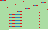
\includegraphics[width=\textwidth,interpolate=false]{fve4.png}
    \caption{Visualization of FVE metadata at the offset of 0xc9c93800 bytes using the \texttt{sweeping} method}
    \label{fig:bitlocker-metadata}
  \end{subfigure}
  \hfill
  \begin{subfigure}[t]{0.45\textwidth}
    \centering
    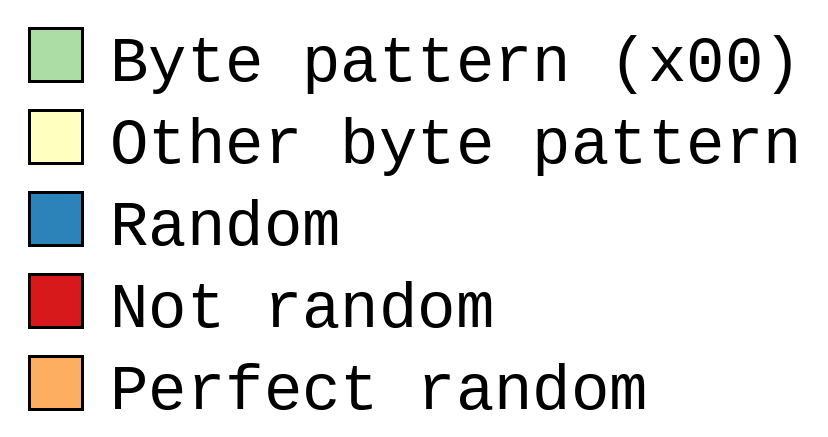
\includegraphics[width=\textwidth]{legend.png}
    \caption{Legend}
    \label{fig:bitlocker-legend}
  \end{subfigure}
  \caption{Windows 10 disk image before and after encryption with BitLocker generated with the \texttt{hilbert-curve} output method and FVE metadata}
  \label{fig:bitlocker}
\end{figure}

In the drive, there are three partitions.
The first is the system partition containing hardware-specific files needed to load windows \cite{winpart}, the second is the data partition visible from windows under the letter C, and the last is the recovery tools partition \cite{winbiospart}.

In the figure \ref{fig:bitlocker-unenc}, one can see that most sectors seem to be unencrypted and, in the figure \ref{fig:bitlocker-enc}, only the first and last partitions remain unencrypted.
After closer inspection, there are also visible chunks of unencrypted sectors in the second partition, and these are sectors containing FVE metadata blocks and their padding \cite{metz22}.
An example of an unencrypted chunk containing FVE metadata can be found in the figure \ref{fig:bitlocker-metadata}. 
For this example, discarding sectors on the drive was not enabled. 
Therefore unused zeroed out sectors are not visible, and it is not easily discernible whether the sector is occupied by a file.

\subsection{Cryptsetup LUKS}
\label{ssec:cryptsetup-luks}

% For this example, the image from the study materials from the year 2019 of the pv204 course\footnote{\url{https://is.muni.cz/auth/el/fi/jaro2019/PV204/um/seminars/08_diskencryption/pv204_fde.zip}} with whole system encryption with LUKS was used.
% The figure FIGURE resulted from converting the image in \texttt{.vdi} to raw format and using the utility.
% In the figure, one can see that only the first part of the image contains chunks of unencrypted sectors.
% Most of the unencrypted part is the boot partition.
% However, after focusing only on the first two megabytes of the encrypted partition, unencrypted sectors, in the beginning, can still be clearly seen.
% This is the LUKS header, and it contains crucial information on decrypting the rest of the partition \cite{faqcryptsetupluks}.

For this example, a cryptsetup LUKS2 mapping was created to a 2GiB file.
After formatting and creating an ext4 filesystem, a Linux kernel was copied into it, after which unused blocks were discarded.
The figure \ref{fig:luks-full} was generated by the utility from the entirety of the 2GiB file.
The figure \ref{fig:luks-header} is generated using the sweeping-blocks method and depicts only the first sixteen megabytes, which is the data from sectors containing the LUKS header.
In the top-left corner, the primary binary header, first JSON area, their padding, and their copy can be seen.
After the second JSON area padding, in accordance with the LUKS2 specification, the cryptographically generated keyslots area follows \cite{broz22}.

% \begin{figure}
%   \centering
%   \begin{subfigure}[t]{.45\textwidth}
%     \centering
%     \includegraphics[width=\textwidth,interpolate=false]{pv204_fde-chi2-4-hilbert.png}
%     \caption{Generated image from the entire disk}
%     \label{fig:idk2-unenc}
%   \end{subfigure}
%   \hfill
%   \begin{subfigure}[t]{.45\textwidth}
%     \centering
%     
\includegraphics[width=\textwidth,interpolate=false]{luks-header.png}
%     \caption{First two megabytes of the encrypted partition}
%     \label{fig:idk2-enc}
%   \end{subfigure}
%   \caption{Whole system encryption with LUKS}
%   \label{fig:idk2}
% \end{figure}
\begin{figure}
  \centering
  \begin{subfigure}[t]{.45\textwidth}
    \centering
    
\includegraphics[width=\textwidth,interpolate=false]{ext4-luks2-sweeping.png}
    \caption{Generated image from the entire 2GiB image using \texttt{sweeping}}
    \label{fig:luks-unenc}
  \end{subfigure}
  \hfill
  \begin{subfigure}[t]{.45\textwidth}
    \centering
    
\includegraphics[width=\textwidth,interpolate=false]{ext4-luks2-head.png}
    \caption{LUKS2 header generated with 8x8 sweeping blocks method}
    \label{fig:luks-full}
  \end{subfigure}
  \begin{subfigure}[b]{.45\textwidth}
    \centering
    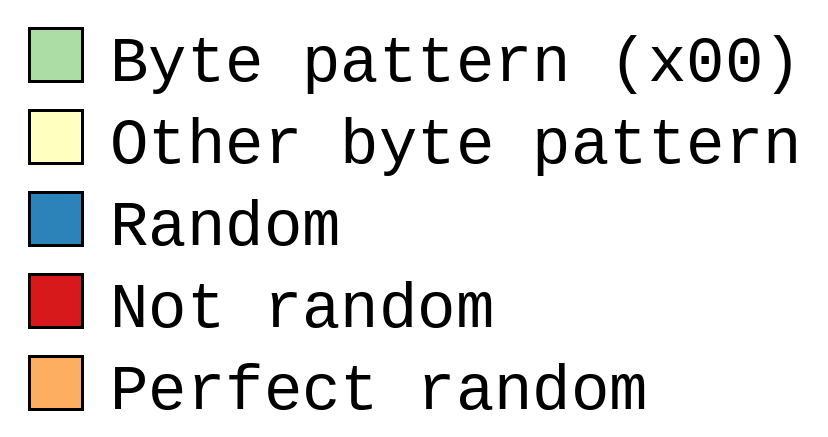
\includegraphics[width=\textwidth]{legend.png}
    \caption{Legend}
    \label{fig:luks-legend} 
  \end{subfigure}
  \caption{LUKS2 full drive encryption}
  \label{fig:luks-header}
\end{figure}

\subsection{VeraCrypt file-hosted volume}
\label{ssec:veracrypt-file-hosted-volume}
A VeraCrypt file-hosted volume of size 1GiB was created in a Ubuntu installation in Oracle VM VirtualBox on a 10GiB virtual drive with ext4 filesystem and without TRIM.
The images in figure \ref{fig:veracrypt} were generated from the converted raw images before and after the VeraCrypt file-hosted volume\cite{veracryptvol} creation.

In the figure \ref{fig:veracrypt-with} is noticeably more sectors marked as \emph{random} than in the figure \ref{fig:veracrypt-without}.
These are the sectors containing the encrypted file. 

However, after a closer inspection, it is clear that the VeraCrypt volume also displaced non-zero byte-pattern sectors.
This could be explained by the fact that some of the displaced sectors classified as not random could be remnants of previously deleted data, which has not been trimmed because of the disabled discard and therefore did not appear as zeroed.

\begin{figure}
  \centering
  \begin{subfigure}[t]{.45\textwidth}
    \centering
    
\includegraphics[width=\textwidth,interpolate=false]{ubnt-unencrypted-chi2-4-sweeping-blocks.png}
    \caption{Without a VeraCrypt volume}
    \label{fig:veracrypt-without}
  \end{subfigure}
  \hfill
  \begin{subfigure}[t]{.45\textwidth}
    \centering
    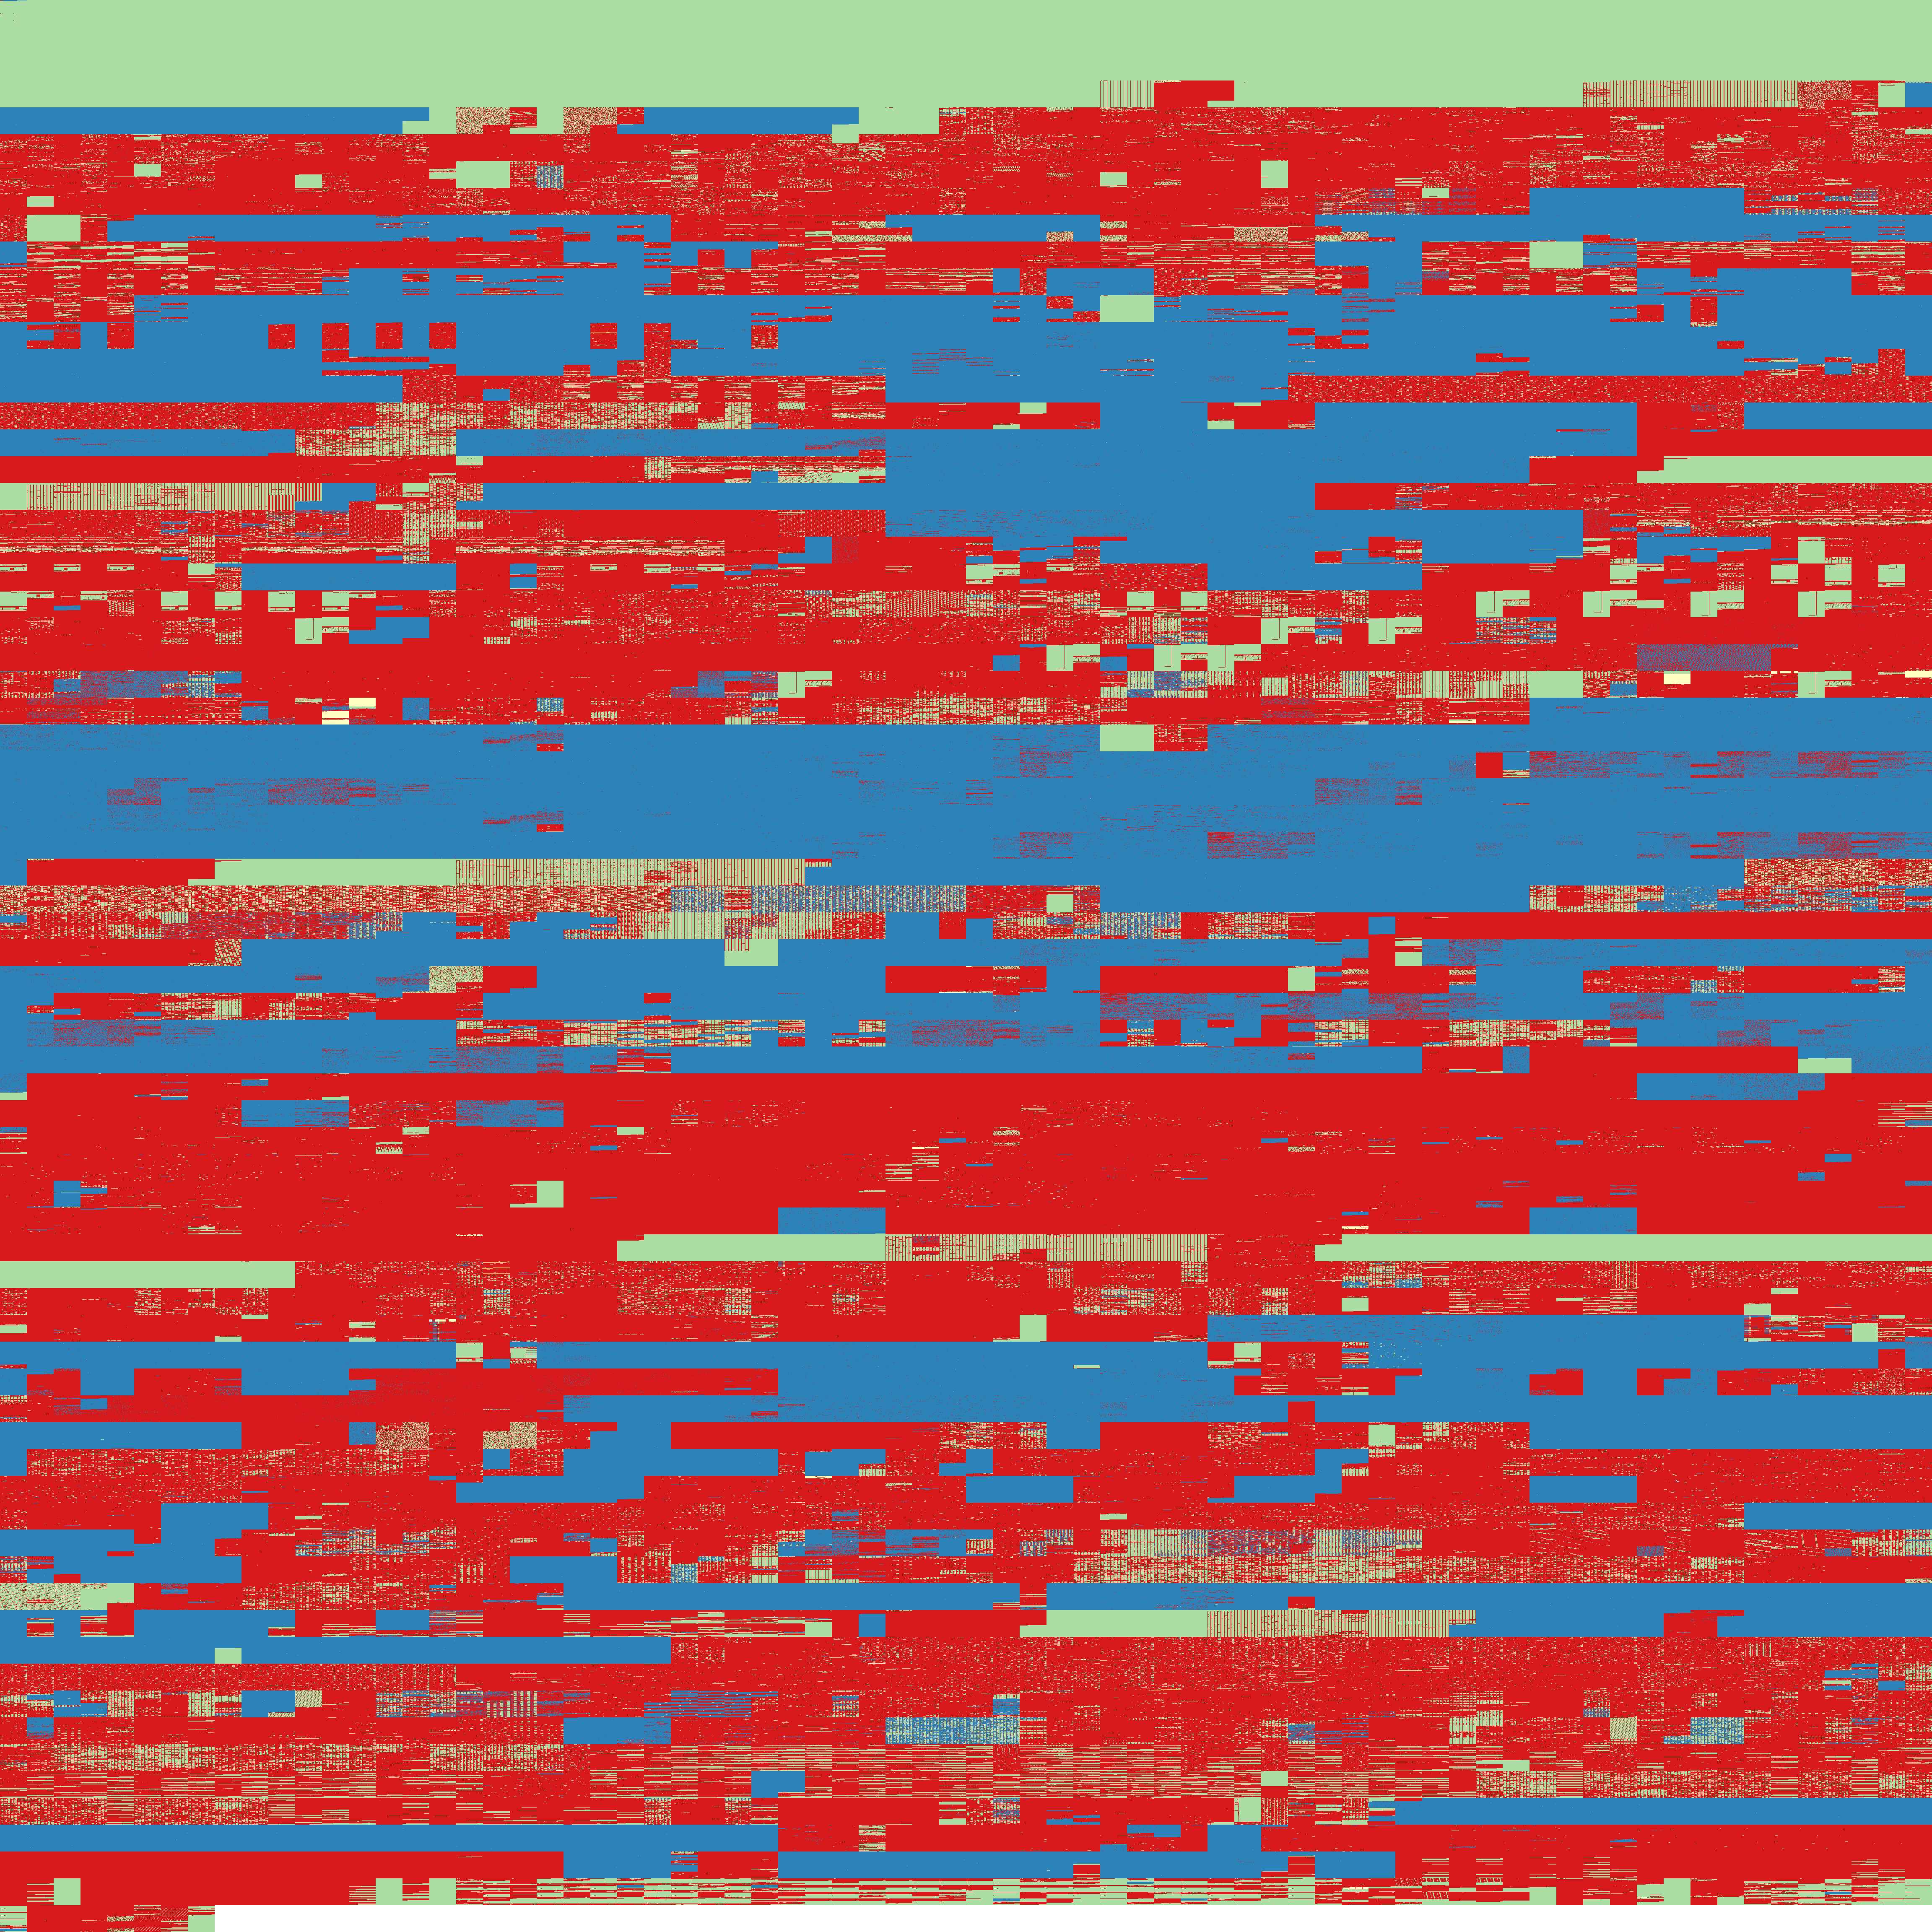
\includegraphics[width=\textwidth,interpolate=false]{ubnt-veracrypt-chi2-4-sweeping-blocks.png}
    \caption{After creating a 1GiB VeraCrypt volume}
    \label{fig:veracrypt-with}
  \end{subfigure}
  \begin{subfigure}[b]{.45\textwidth}
    \centering
    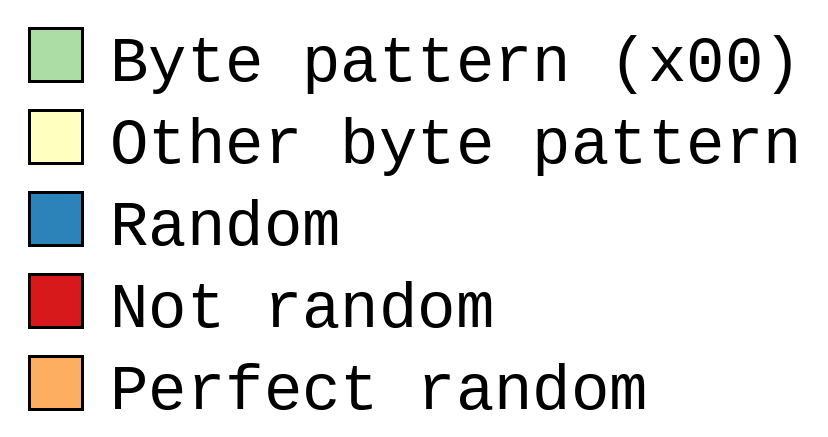
\includegraphics[width=\textwidth]{legend.png}
    \caption{Legend}
    \label{fig:veracrypt-legend} 
  \end{subfigure}
  \caption{Difference before and after creating a VeraCrypt file-hosted volume generated by the  \texttt{sweeping-blocks} method}
  \label{fig:veracrypt}
\end{figure}

\chapter{Conclusion}
\label{chap:conclusion}

In this thesis, algorithms for the analysis of sector patterns were described.
This thesis also described orders of pixel placements for the visualization of the analysis results and also introduced one.
A utility was implemented which incorporates these algorithms for disk sector analysis and visualization of the results and is available on GitHub\footnote{\url{https://github.com/malon43/entropy-visualization}} under the MIT license.
The utility allows for multiple output methods, including images and CSV files.
The generated CSV file can later be transformed using any implemented method using the \texttt{from\_csv.py} script without the need for running the time-intensive analysis multiple times only for using multiple output methods on the same input. 

This utility was then used to analyze and visualize various disk images, and in the chapter \ref{chap:results}, the results were discussed.

\section{Future work}
\label{sec:future-work}

Possible future extensions or modifications of the utility include:
\begin{itemize}
  \item optimizing the existing analysis methods for faster analysis
  \item adding new analysis and output methods or new palettes
  \item incorporating analysis of byte patterns at specific offsets of the image
  \item options to incorporate filesystem information to classify used sectors based on which file's contents they store
  \item adding an analysis progress indicator
\end{itemize}

\makeatletter\thesis@blocks@clear\makeatother
\sloppy
\printbibliography

\appendix %% Start the appendices.
\chapter{Utility usage}
\label{chap:utility-usage}

\begin{verbatim}
usage: script.py [-h] [-s SIZE] [-m OUTPUT_METHOD] 
                 [-a ANALYSIS_METHOD] 
                 [-l SIG_LEVEL | 
                 [--rand-lim RAND_LIM 
                  --sus-rand-lim SUS_RAND_LIM]]
                 [output method arguments] DISK_IMAGE

options:
  -h, --help            show this help message and exit
  -s SIZE, --size SIZE  set the sector size (default:
                        512)
  -m OUTPUT_METHOD, --method OUTPUT_METHOD
                        set the output method
                        (available: sample-output, csv,
                        sweeping, sweeping-blocks,
                        hilbert-curve) (default:
                        sweeping)
  -a ANALYSIS_METHOD, --analysis ANALYSIS_METHOD
                        set the analysis method
                        (available: shannon, chi2-8,
                        chi2-4, chi2-3, chi2-1, kstest)
                        (default: chi2-4)
  -l SIG_LEVEL, --significance-level SIG_LEVEL
                        the significance level to use
                        for classification (cannot be
                        used with 'rand-lim' and 'sus-
                        rand-lim') (default: 0.0002)
  --rand-lim RAND_LIM   random significance limit
                        (default: 0.9999)
  --sus-rand-lim SUS_RAND_LIM
                        randomness suspiciously high
                        significance limit (default:
                        0.0001)


  sample-output:
    --output-file OUTPUT_FILE
                          output file (default: stdout)
    --err-file ERR_FILE   error output file (default:
                          stderr)
    --entropy-limit ENTROPY_LIMIT
                          omits every sector the entropy
                          of which is higher than the
                          provided value (default: inf)

  csv:
    --output-file OUTPUT_FILE
                          output file (default: stdout)
    --err-file ERR_FILE   error output file (default:
                          stderr)
    --entropy-limit ENTROPY_LIMIT
                          omits every sector the entropy
                          of which is higher than the
                          provided value (default: inf)
    --no-header           the resulting csv file will not
                          contain a header
    --separator SEPARATOR
                          sets the provided string as a
                          separator of the csv file
                          (default: ',')

  sweeping:
    --output-file OUTPUT_FILE
                          output file (default: stdout)
    --err-file ERR_FILE   error output file (default:
                          stderr)
    --no-legend           resulting image will not
                          contain a legend
    --background BACKGROUND
                          hex code of background color
                          (default: white)
  

    --palette PALETTE     color palette to use
                          (available: asalor, sample, rg,
                          photocopy-safe) (default:
                          photocopy-safe)
    --font FONT           font to use for legend
                          (default: LiberationMono-
                          Regular)
    --font-size FONT_SIZE
                          font size to use for legend in
                          pixels (default: automatic)
    --font-color FONT_COLOR
                          hex code of font color of the
                          legend (default: automatic)
    --width WIDTH         the width of the resulting
                          image in pixels (default:
                          automatic square)

  sweeping-blocks:
    --output-file OUTPUT_FILE
                          output file (default: stdout)
    --err-file ERR_FILE   error output file (default:
                          stderr)
    --no-legend           resulting image will not
                          contain a legend
    --background BACKGROUND
                          hex code of background color
                          (default: white)
    --palette PALETTE     color palette to use
                          (available: asalor, sample, rg,
                          photocopy-safe) (default:
                          photocopy-safe)

    --font FONT           font to use for legend
                          (default: LiberationMono-
                          Regular)
    --font-size FONT_SIZE
                          font size to use for legend in
                          pixels (default: automatic)
    --font-color FONT_COLOR
                          hex code of font color of the
                          legend (default: automatic)
    --width WIDTH         the width of resulting image in
                          pixels (default: automatic
                          square)
    --sweeping-block-size SWEEPING_BLOCK_SIZE
                          the size of block groups of the
                          resulting image (default:
                          automatic)

  hilbert-curve:
    --output-file OUTPUT_FILE
                          output file (default: stdout)
    --err-file ERR_FILE   error output file (default:
                          stderr)
    --no-legend           resulting image will not
                          contain a legend
    --background BACKGROUND
                          hex code of background color
                          (default: white)
    --palette PALETTE     color palette to use
                          (available: asalor, sample, rg,
                          photocopy-safe) (default:
                          photocopy-safe)
    --font FONT           font to use for legend
                          (default: LiberationMono-
                          Regular)
    --font-size FONT_SIZE
                          font size to use for legend in
                          pixels (default: automatic)
    --font-color FONT_COLOR
                          hex code of font color of the
                          legend (default: automatic)
\end{verbatim}
\end{document}
